
\documentclass[12pt]{harvardalmthesis}
\listfiles

%% personal customizations like graphics, math, ...
%% This file contains personal customizations like graphics, math,
%% algorithm/code listing, and glossary.


% ------------------------------------------------------------
% graphics

\usepackage{graphicx}
\usepackage{epsf}
\usepackage{multicol}
\usepackage{graphics,color,latexsym}



%% ------------------------------------------------------------
%% basic math packages

\usepackage{amsmath}
\usepackage{amssymb}
\usepackage{amsthm}
\usepackage{amsfonts}
\usepackage{theorem}

% other math packages
\usepackage{bm}

% for diagrams
\usepackage{amscd}

% for conditionals
\usepackage{ifthen}

% linear
%\usepackage{esvect}

\usepackage{enumerate}

% change the way items are numbered in the enumerate environment
\renewcommand{\labelenumi}{(\alph{enumi})}

%% ------------------------------------------------------------
%% some basic math definitions


%% ------------------------------------------------------------
%% some math environments


\newlistof{myequations}{equ}{\listequationsname}
\newcommand{\addmyequations}[1]{
  \addcontentsline{equ}{myequations}{\protect\numberline{\theequation}#1}\par
}
\cftsetindents{myequations}{1.5em}{3em}


%% ------------------------------------------------------------
%% some math bold faces



%% ------------------------------------------------------------
%% for some CS

%\def\O{\mathcal{O}}

\newcommand{\sym}[1]{\texttt{#1}}
\newcommand{\algor}[1]{\textsf{\textsc{#1}}}


% ------------------------------------------------------------
% for code and algorithms 

\usepackage{verbatim}
\usepackage[chapter]{algorithm}
\usepackage{listings}
%\usepackage{algorithmic}
\usepackage{afterpage}		% help with multi-page listing



\newcommand{\INPUT}{\textbf{Input}}
\newcommand{\as}{\ensuremath{\leftarrow}}

% these should be after hyperref because of conflicts
% this might help
%\newcommand{\theHalgorithm}{\arabic{algorithm}}

% for lsting
%\renewcommand{\lstlistingname}{\textbf{Algorithm}}
%\renewcommand{\lstlistlistingname}{Algorithms}


\lstdefinelanguage{Algorithm}%
{morekeywords={input,for,each,while,if,else,then,do,to,break,end,print,return,function},%
  aboveskip=\smallskipamount,
  belowskip=\smallskipamount,
  xleftmargin=25pt,         
  basicstyle=\footnotesize,	% \tiny, \scriptsize, \small, \footnotesize, \bfseries, \upshape
  sensitive,%
  mathescape,%
  commentstyle=\footnotesize\upshape,%
%  morecomment=[s]{\{}{\}},%
  morecomment=[s]{\{}{\}},%
  %morecomment=[l]\%,%
  %morestring=[m]'%  
%  fontadjust=true,		%
  texcl=true,			% include TEX source
  numbers=left,			% where to put the line-numbers
  numberstyle=\tiny,		% 
  numbersep=10pt,		% how far the line-numbers are from the code
  captionpos=b,		        % sets the caption-position to bottom
 }


\lstdefinelanguage{JavaText}%
{
  aboveskip=\smallskipamount,
  belowskip=\smallskipamount,
  xleftmargin=25pt,         
  basicstyle=\footnotesize\ttfamily,	% \tiny, \scriptsize, \small, \footnotesize, \bfseries, \upshape
  frame=single,			% adds a frame around the code ('single', 'b')
  numbers=left,			% where to put the line-numbers
  numberstyle=\tiny,		% 
  numbersep=10pt,		% how far the line-numbers are from the code
  captionpos=b,		        % sets the caption-position to bottom
}
\lstdefinelanguage{Java}%
{
}


\lstdefinelanguage{XMLText}%
{
  aboveskip=\smallskipamount,
  belowskip=\smallskipamount,
  xleftmargin=25pt,         
  basicstyle=\footnotesize\ttfamily,	% \tiny, \scriptsize, \small, \footnotesize, \bfseries, \upshape
  frame=single,			% adds a frame around the code ('single', 'b')
  numbers=left,			% where to put the line-numbers
  numberstyle=\tiny,		% 
  numbersep=10pt,		% how far the line-numbers are from the code
  captionpos=b,		        % sets the caption-position to bottom
}
\lstdefinelanguage{XML}%
{
  basicstyle=\footnotesize\ttfamily,	% \tiny, \scriptsize, \small, \footnotesize, \bfseries, \upshape
}



%% The default listing format
%% 
\lstset{ %
  %language=Java,		% default language, set with \lstset{language=XXX}
  %------- MARGINS and FRAMES --------
%  aboveskip=\smallskipamount,
%  belowskip=\smallskipamount,
  xleftmargin=0pt,         
  % xleftmargin=17pt,
  %framexleftmargin=17pt,
  %framexrightmargin=5pt,
  %framexbottommargin=4pt,
  % frame=single,			% adds a frame around the code ('single', 'b')
  % float=true,			% make it a float
  %------- FONTS --------
  basicstyle=\footnotesize\ttfamily,	% \tiny, \scriptsize, \small, \footnotesize, \bfseries, \upshape
  % keywordstyle=\bfseries,	% \color{red},
  % commentstyle=\upshape,	%         
  % stringstyle=\color{white}\ttfamily,	%
  %------- BACKGROUND COLOR --------
  %backgroundcolor=\color{white},  % choose the background color. Must add \usepackage{color}
  %backgroundcolor=\color{lightgray},
  %------- HORIZONTAL SPACING  --------
  % fontadjust=true,		%
  keepspaces=true,		%
  showspaces=false,		% show spaces adding particular underscores
  showstringspaces=false,	% underline spaces within strings
  showtabs=false,               % show tabs within strings adding particular underscores
  % tabsize=3,			% sets default tabsize to 2 spaces
  columns=[l]flexible,		% 'flexible', 'fixed'
  % texcl=true,			% include TEX source
  %------- NUMBERING --------
  numbers=none,			% where to put the line-numbers
  %numberstyle=\tiny,		% 
  %numbersep=10pt,		% how far the line-numbers are from the code
  % stepnumber=2,		% the step between two line-numbers. If it's 1 each line will be numbered
  %------- CAPTION --------
  % caption=\lstname		% default caption name
  %captionpos=b,		% sets the caption-position to bottom
  %------- LINE BREAKING --------
  breaklines=true,		% sets automatic line breaking
  % breakatwhitespace=false,    % sets if automatic breaks should only happen at whitespace
  %------- COMMENTS --------
  % escapeinside={\%*}{*)}          % if you want to add a comment within your code
}

%\cftsetindents{algorithm}{1.5em}{3em}

%\renewcommand{\lstlistingname}{Listing \arabic{chapter}.\arabic{section}}




% ------------------------------------------------------------
% for url
\usepackage{url}

\usepackage[pdftex,colorlinks,plainpages=false,pdfpagelabels]{hyperref}
%\usepackage[ps2pdf=true,colorlinks]{hyperref}
%\usepackage{hyperref}	%% this should be last

\usepackage[figure,table]{hypcap} % Correct a problem with hyperref
\hypersetup{
% these are from beamer
  bookmarks=true,%
%  bookmarksopen=true,%
  pdfborder={0 0 0},%
  pdfhighlight={/N},%
  linkbordercolor={.5 .5 .5},
%%
  bookmarksnumbered,
  pdfstartview={FitH},
  citecolor={black},
  linkcolor={black},
  urlcolor={black},
  pdfpagemode={UseOutlines}
} 
\makeatletter
\newcommand\org@hypertarget{}
\let\org@hypertarget\hypertarget
\renewcommand\hypertarget[2]{%
  \Hy@raisedlink{\org@hypertarget{#1}{}}#2%
} \makeatother 

% ------------------------------------------------------------
% Glossary

\usepackage{etex}   % to avoid: 'supp-mis.tex:197: No room for a new \dimen'
%\usepackage[nonumberlist,section=chapter,numberedsection=autolabel]{glossaries}
\usepackage[section=chapter,numberedsection=autolabel]{glossaries}

%% make glossary
% latex
% makeindex -s main.ist -t main.glg -o main.gls main.glo
% ./makeglossaries.pl main
% latex; latex

% for glossary
\makeglossaries
\loadglsentries{glossary}

% load all glossary entries
%\glsaddall

%A \gls{sample} entry and \gls{aca}. Second use: \gls{aca}.
%Plurals: \glspl{sample}. Reset acronym\glsreset{aca}.
%First use: \glspl{aca}. Second use: \glspl{aca}.


%% ------------------------------------------------------------
%% OTHER CUSTOMIZATIONS

% for landscape pages
\usepackage{lscape}

\DeclareGraphicsExtensions{.pdf,.eps,.jpg,.mps,.png}

\usepackage{pifont}





\begin{document}

% ------------------------------------------------------------
% BEGINNING PART

%% Roman numeral page counting
\pagenumbering{roman}
\setcounter{page}{1}

\pdfbookmark[0]{Titlepage}{title}

\thispagestyle{empty}
\begin{center}

  % Title  Two inches from the top of the page
  \vspace*{0.6in}
  Socrates Sim: A User Simulator to Support Task Completion Dialog Research
  
  % Full Name  2.5 inches below the first line of the Title
  \vspace{2.3in}
  Dhairya Dalal\\
  \vspace{1.8in}
  A Thesis in the Field of Software Engineering\\
  for the Degree of Master of Liberal Arts in Extension Studies\\
  \vspace{.8in}
  Harvard University\\

  % Graduation Date, 2.5 inches from the bottom, e.g., November 2004
  \vfill
  August 2018
  \vspace*{.5in}
\end{center}




%%% Local Variables: 
%%% mode: latex
%%% TeX-master: "main"
%%% End: 



%% Blank page
\clearpage
%\phantomsection % Ensures that a PDF bookmark is set here
%\pdfbookmark[0]{}{}
\chapter*{}
\thispagestyle{empty}	% no page numbering



\clearpage
%\phantomsection % Ensures that a PDF bookmark is set here
\pdfbookmark[0]{Abstract}{abstract}
\chapter*{Abstract}
\thispagestyle{empty}	% no page numbering

In this thesis, we propose an end-to-end dialog simulation framework, called Socrates Sim, to support task-completion dialog research. The goal of the framework is to provide a set of tools that will simulate generate between a user simulator and a dialog agent in order to evaluate the performance of the dialog agent and generate annotated data. Specifically, the Socrates Sim framework allows the researcher to define the custom dialog domains, build user simulators, and run multiple simulations with a provided dialog agent. To demonstrate the flexibility of the framework to generalize to new domains, implement end-to-end simulations in the following domains: restaurant recommendations and movie bookings. The framework is implemented in Python 3.6 and made available on GitHub (https://github.com/dhairyadalal/socrates). 

%%% Local Variables: 
%%% mode: latex
%%% TeX-master: "main"
%%% End: 



\clearpage
%\phantomsection % Ensures that a PDF bookmark is set here
\pdfbookmark[0]{Acknowledgements}{acknowledgements}

\chapter*{Acknowledgments}

This project was  able to be completed due to the support and guidance of many wonderful individuals in my life. I would like to first thank Professor Stuart Shieber for serving as my thesis adviser. I would not have able to complete this ambitious project without your support and guidance. 

Additionally, I would like to thank my supervisors Byron Galbraith, Paula Long, and the Talla organization for their patience and support as I undertook this project. I was a full-time employee for Talla while working writing and researching this thesis. Balancing the demands of work while researching was challenging. I am incredibly fortunate to work for an organization that provided me with the flexibility to take time off and prioritize the completion of my degree and this thesis. Without that support, this project could not have been completed.

The idea for this project initially arose from my time at the Allen Institute for Artificial Intelligence (AI2). Vu Ha, Amos Ng and I were the part of a team that was exploring novel research areas in the dialog space. This project was initially slated to be AI2's fifth research track but was quickly decommissioned after AI2 chose to prioritize other research. I greatly appreciate the blessing from Vu Ha and AI2 to be able to continue the project independently. 

This degree has taken quite a long time to complete. I started the ALM program in 2013 while working full time at Harvard. Over the course of this program, I've changed my job four times, moved across the country to Seattle and back to Cambridge. While it has been exhausting and demanding, I have had profound emotional support from my family and friends. I am grateful to mother (Shobha), father (Bharat), and sister (Dhara) for continuing to nag, push, and of course provide generous amounts of love and encouragement. I am also thankful for my dear friend and partner Camille Shaw who sent pictures of cute animals daily to motivate me and provided so much emotional support. And finally, thank you Thakurji for blessing me and providing opportunities for success.  


%%% Local Variables: 
%%% mode: latex
%%% TeX-master: "main"
%%% End: 


\clearpage
\phantomsection % Ensures that a PDF bookmark is set here
%\pdfbookmark[0]{Contents}{contents}
\addcontentsline{toc}{chapter}{Table of Contents}
\tableofcontents


\clearpage
\phantomsection
\addcontentsline{toc}{chapter}{List of Figures}
\listoffigures

\clearpage
\phantomsection
\addcontentsline{toc}{chapter}{List of Tables}
\listoftables

\clearpage
\phantomsection
\addcontentsline{toc}{chapter}{List of Equations}
\listofmyequations
%\listofmyequations

\clearpage
\phantomsection
\addcontentsline{toc}{chapter}{List of Algorithms}
\listofalgorithms


\clearpage
\phantomsection
\addcontentsline{toc}{chapter}{List of Code}
\renewcommand{\lstlistlistingname}{List of Code}
\lstlistoflistings



%% ------------------------------------------------------------
%% MAIN PART

%% Restarting page counting with numeric
\clearpage
\pagenumbering{arabic}
\setcounter{page}{1}


\chapter{Introduction}

\section{Project Goals}

In this thesis, we present an end-to-end dialog simulation framework called Socrates Sim, which supports task-completion dialog research. The goal of our framework is to provide a set of tools that simulate conversations between a user simulator and a dialog agent in order to evaluate the performance of the dialog agent and generate annotated data. Specifically, Socrates Sim allows researchers to define the custom dialog domains, build user simulators, and run multiple simulations with a provided dialog agent with a single unified framework. 

Task-completion dialog agents have grown in popularity in the past few years. With the advent of home assistant services like Amazon's Alexa and advances in dialog research, there has been a rise in the development of dialog agents that provide various user services like flight bookings and restaurant recommendations. One of the key challenges in developing these agents is the effective training and evaluation of them. There are only a handful of tools available to support dialog research. Missing in this space is a framework that facilitates end-to-end simulation between a user simulator and dialog agent. There are several value propositions for such a framework.

One of the main challenges is that it is very expensive to train dialog agents and produce quality training data. It is a very labor intensive and human-centric process. User simulators can alleviate the need for human testers by simulating human behavior. A framework that simulates the conversation between a user simulator and dialog agent can be used to generate large amounts of ancillary data to augment manually collected training data for model-based dialog agents. Additionally, our framework provides a standardized way to test the robustness and efficacy of a dialog agent.

The intended users of this framework are academic researchers and data scientists or software engineers in industry. The framework is modular and retargetable to support multiple domains. This makes it easy for the researcher to build and test different user simulators for their dialog agent and produce diverse datasets. 

In this thesis, our focus is on the design and implementation of the Socrates Sim framework. We use as inspiration the framework architecture described in \cite{li_usersim} and the configuration based approach used by \cite{Gardner_allennlp} for AllenNLP. The primary limitation of the \cite{li_end_to_end} framework is that it tightly couples the user simulator with the development of a dialog agent. As a result, adapting the framework to a new domain requires reimplementing the entire architecture. 

Our contribution is the design and implementation of a framework that generalizes to new domains in a scalable manner. We abstract and modularize key components in order to develop a framework that is domain independent. The researcher can plug in different dialog agents and user simulators in order to run simulations, evaluate the agent, and generate annotated training data. Additionally, we make the framework easier to use by utilizing a configuration based approach, in which the user specifies the simulation parameters in an external configuration file. The user can set up multiple experiments, change domains, dialog agents, and user simulators without having to write new code or manually provide component locations as a long list of command line parameters. Finally, our framework scales efficiently as the number of simulations it generate increases. 

The framework consists of the following components:
\begin{itemize}
	\item \textbf{Dialog Domain}: A set of classes to represent the dialog domain and knowledge base. The dialog domain consists of all possible dialog acts, valid inform/request slots and values, and other domain specific information. 
	\item \textbf{Speaker Interface}: A unified interface that defines a standardized protocol for the external user simulators and dialog agent to communicate with the framework. 
	\item \textbf{Dialog Manager}: A coordinator tool that facilitates the conversation between the user simulator and dialog agent. Additionally, the dialog manager tracks simulation histories, evaluates simulated dialogs, and serializes annotated simulations to disk.  
\end{itemize}

In the next section, we provide more background on the evolution of task-completion dialog research and the motivation for developing Socrates Sim. 

\section{Background}

Task-completion dialog refers to the space of dialog activities in which an end user engages with an interlocutor in order to complete a task or achieve a tangible goal. For example, imagine a user interacting with a concierge in order to identify and book a restaurant for dinner. In dialog systems, the human interlocutor is replaced by an artificial agent (also referred to as the system or dialog agent) that can intelligently respond and help the user achieve their goal.

Automated dialog systems are not a new concept. They have been used to support call routing (e.g. press 1 to reach sales) in the context of customer support for banks, credit cards, flight booking, and many other commercial sectors since the 1970s. Central to any dialog system is the dialog policy. The dialog policy informs the system on what to say and what information to collect based on the state of the conversation. Traditionally dialog policies were scripted out, usually following a simple flowchart-like structure. This is known as a rules-based approach, where rules are written out to capture system behavior in predefined situations/states. Rules-based systems are limited in that they require the user to follow a scripted path and provide the system with one piece of information at a time. While effective, many users are often frustrated with rules-based dialog systems and tend to prefer speaking to a human agent. Much of this frustration is caused by the slow pacing of the dialog scripts, which require the user to specify information individually and in a specific order. 

There has been significant progress in the AI and machine learning space that has led to the development of commercially viable intelligent dialog systems. In particular, the popularity of voice assistants like Amazon's Alexa, Apple's Siri, and Google's Assistant have increased the demand for voice interfaces to popular applications and services. There has been a boom in the development of chatbots, third-party voice skills for Alexa and Google Home, and other dialog based services. Much of this is due to the proliferation of exciting research which applies deep learning and machine learning to the dialog domain. 

However, developing good voice interfaces and dialog systems is still very challenging. For example, a significant proportion of the voice skills in the Alexa skills store have poor ratings \cite{rey_2017}. According to research by recode.com, 69\% of skills in the Alexa skill store have a 0 or 1  star reviews, suggesting abysmal usage. In addition, there is only a 3\% chance that a user will reuse a voice skill after the first use, demonstrating poor retention. Underlying these poor statistics is the fundamental challenge - designing robust and usable dialog systems is very difficult. 
 
Rules-based dialog systems neither scalable nor optimal for more complex task completion. Researchers have moved to leverage supervised learning (SL) methods to train dialog systems and produce more robust dialog policies. In an SL approach, the dialog policy is trained to imitate the observed actions of an expert using annotated and manually crafted datasets based on real human interactions \cite{Schatzmann2006ASO}. While this approach produces better policies than a rules-based approach, it is limited by the quality and scope of the training data. 

One of the key challenges in this space is developing quality and diverse training data. Producing deep annotated data is time-consuming and expensive. The dataset may not comprehensively cover all possible states in a policy space. Supervised learning requires large amounts of clean and annotated training data. This involves having many human testers interacting with a human expert (which proxies for the dialog agent) in order to generate what the ideal conversations would look like. In response to user questions and actions, the human expert would choose the correct policy from a defined action space. Over the course of the dialog, the human expert identifies all the right actions that will eventually lead to helping the user accomplish their goal. This process is repeated across many users in order to capture the different goals a user may have and how they communicate. Current data gathering practices rely on crowd-sourcing and general human trials. While these approaches are effective at generating high-quality data, they are incredibly expensive and limited in how they can capture information.  

Reinforcement learning (RL) methods are also gaining popularity. Given a reward function, the agent can optimize a dialog policy through interaction with users and learn what an optimal dialog policy should be. Reinforcement learning approaches are more robust than supervised learning techniques as the agent can explore more of the policy space.

A virtual simulator could alleviate these data needs by simulating a user in place of using a real human user. The user simulator can be used in the context of supervised learning (SL) or reinforcement learning (RL) to train a dialog system on how to identify optimal policies. The simulator would generate additional synthetic data to help augment the training data acquired through human testing. The user simulator would also provide a useful starting point to train RL based agents, which then can be further optimized in RL situation with real users \cite{li_usersim}. Currently there is no open source or commercially available framework to support end-to-end simulations with user simulators. The aspiration of this thesis is to develop a solution that can fill that gap. 

\section{Prior Work}
\label{sec:priorworks}

The growing popularity of statistical approaches for spoken dialog systems has led to research for more optimal ways to generate training data. \cite{Schatzmann2009TheHA} introduced the concept of the hidden agenda user simulation model, which has been foundational to conceptualizing user simulators. Schatzmann and Young provide a formalized framework to capture user intents in a stack-like structure of pending dialog acts. \cite{BordesW16} applied deep learning and neural models to dialog systems. They introduced the concept of a neural network-based end-to-end trainable dialog system. Their approach treats dialog system learning as problem learning and attempts to map dialog histories to system responses by applying encoder-decoder models for training. 

\cite{li_usersim} developed a framework for a user simulator and released a research proof of concept which was applied to the movie booking domain. They released a proof-of-concept framework, TC-Bot. The framework was written in Python 2.7 and hard-coded to support the movie booking domain. Currently, there is no open source and modern user simulator tool for task-completion dialog research. Our framework is written in Python 3.6.0 and applies good software engineering principles. It is our aspiration that Socrates Simulator can be used for other domains by the dialog research community. 

Finally, Facebook recently released the beta version ParlAI. ParlAI aims to provide a standardized and unified framework for developing dialog models. They have released a broad set of tools to support training and development of dialog systems for the following domain areas: question answering, goal oriented dialog, chit-chat dialog, visual QA/dialog and sentence completion. ParlAI offers a simplified set of API calls to common dialog datasets (e.g. SQuAD, bAbI tasks, MCTest, etc) and provides a set of hooks to Amazon's Mechanical Turk to test one’s dialog model against real human testers. While ParlAI offers an expansive set of tools and datasets, missing from its framework is support for incorporating user simulators. 

\section{Thesis Overview}

In this thesis, we describe the architecture of Socrates Sim, provide implementation details for two different domains, and demonstrate our framework usability through a set of runtime performance evaluations. In chapter 2, we describe the architecture of the Socrates Sim framework. In particular, we focus on modeling conversations, how to standardize communication between external dialog agents and user simulators, and the underlying dialog management framework. 

In chapter 3, we describe the general implementation process for setting up and using Socrates Sim. In chapters 4 and 5, we specifically explore how Socrates Sim was adapted to support the restaurant and movie domains. We detail the development of user simulators, dialog agents, and the underlying dialog components for both domains. Additionally, we highlight the use of configuration files that allow for rapid experimentation and easy swapping of modular components without having to modify existing code. 

In chapter 6, we describe the development of Socrates Sim and cover the tools, language, and other programming specific choices made in developing Socrates Sim. In chapter 7, we provide evidence that Socrates Sim is usable and efficient. Multiple performance tests were run to evaluate the runtime efficiency and memory consumption of Socrates Sim as it ran an increasing number of simulations. We used TC-Bot (\cite{li_end_to_end}) as a benchmark to evaluate performance. We show how Socrates Sim scales efficiently and maintains shallow linear growth for it runtime execution.

Finally, in chapter 8, we conclude this thesis. We describe known limitations, talk about the lessons learned, and provide suggestions for future work.

%%% Local Variables: 
%%% mode: latex
%%% TeX-master: "main"
%%% End: 




\chapter{Requirements}
\label{chap:requirements}

%\section{Introduction}
%\label{sec:workflowexample}

This chapter specifies the requirements of the system.  


\section{High-level Requirements}
\label{sec:requirements}


\section{System Functionality}
\label{sec:systemfunction}


%%% Local Variables: 
%%% mode: latex
%%% TeX-master: "main"
%%% End: 



\chapter{Design}
\label{chap:design}

\section{Overview}
\label{sec:designintroduction}

In this chapter, we describe the architecture of the Socrates Sim framework, highlight key design choices, and describe in detail the component parts. Our goal is to develop a modularized and production-grade dialog simulation framework that can be re-targeted for new domains, produce training data and evaluate dialog agents. The overall design for the simulator was inspired by the work done by \cite{li_usersim}. For the user simulator, we implement the theoretical formulation of the hidden user agenda models described in \cite{Schatzmann2009TheHA}. We also adopt the configuration first user access pattern used in the AllenNLP library \cite{Gardner_allennlp}.

At a high level, Socrates Sim consists of the following components:
\begin{itemize}
	\item \textbf{Dialog Domain}: A set of classes to represent the dialog domain and knowledge base. The dialog domain consists of all possible dialog acts, valid inform/request slots and values, and other domain-specific information. 
	\item \textbf{Speaker Interface}: A unified interface that defines a standardized protocol for the external user simulators and dialog agent to communicate with the framework. 
	\item \textbf{Dialog Manager}: A coordinator tool that facilitates the conversation between the user simulator and dialog agent. Additionally, the dialog manager tracks simulation histories, evaluates simulated dialogs, and serializes annotated dialogs to disk.  
\end{itemize}


\section{Architecture and Design} 

The general architectural is greatly inspired by the end-to-end neural dialog framework described in \cite{li_end_to_end}  (see Figure \ref{fig:li_end_end}). In this design, there are two key components. The first is an agenda based user simulator, which has an internal natural language generation (NLG) model. The right-hand side of the framework is the Neural Dialog System, which consists of a language understanding (LU) unit and a dialog management (DM) unit. The user simulator generates speech utterances using its NLG and sends to the LU unit. The LU parses the speech utterance into a semantic frame (implemented as Python dictionary) and hands it the dialog management unit, which generates a system action and sends to the user simulator (as a semantic frame). The dialog manager also has a state tracker and policy learner. The policy learner is implemented as a deep Q-network (DQN). 

\begin{figure}[h!]
	\label{fig:li_end_end}
	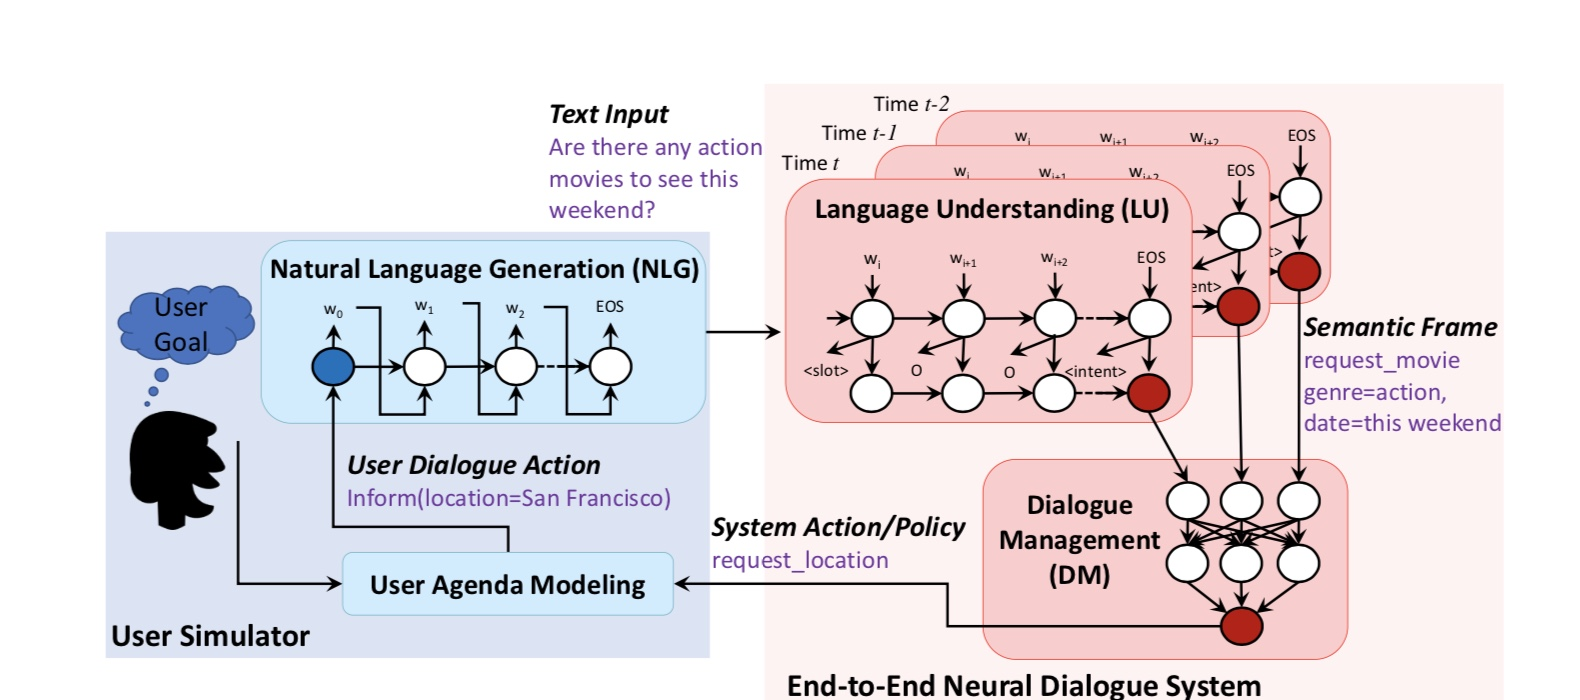
\includegraphics[width=\linewidth]{diagrams/li_end_to_end.jpeg}
	\caption{ The user simulator architecture described by Li et al. (2016) }
\end{figure}

The neural dialog system uses reinforcement learning to learn optimal policies for the dialog agent. At the end of each simulated conversation, the dialog manager will score itself and update its policy learner. One of the key limitations of this approach is that the dialog agent is built in as a learner in the Neural Dialog System. After a set of predefined rounds, the output will be a neural dialog agent serialized as a model file. The simulated dialogs will also be stored externally and can be used downstream as further training data.

The primary challenge with this framework is that it difficult to adapt it to new domains. While the user simulator is a separate component and can be easily reconfigured, the dialog agent and dialog manager are tightly coupled. The dialog agent must be implemented as a neural learner. To adapt this framework to a new domain would require rewriting the dialog manager, language understanding unit, and the surrounding scaffolding scripts which set up and run the simulations. In the research code provided by \cite{li_end_to_end}, the domain information (movie booking) is directly hardcoded into all the aspects of the framework. Communication between components takes place with Python dictionaries, which can be defined arbitrarily. This introduces an element of variability that can present challenges downstream for debugging.

\begin{figure}[h!]
	\label{fig:socrates_sim_framework}
	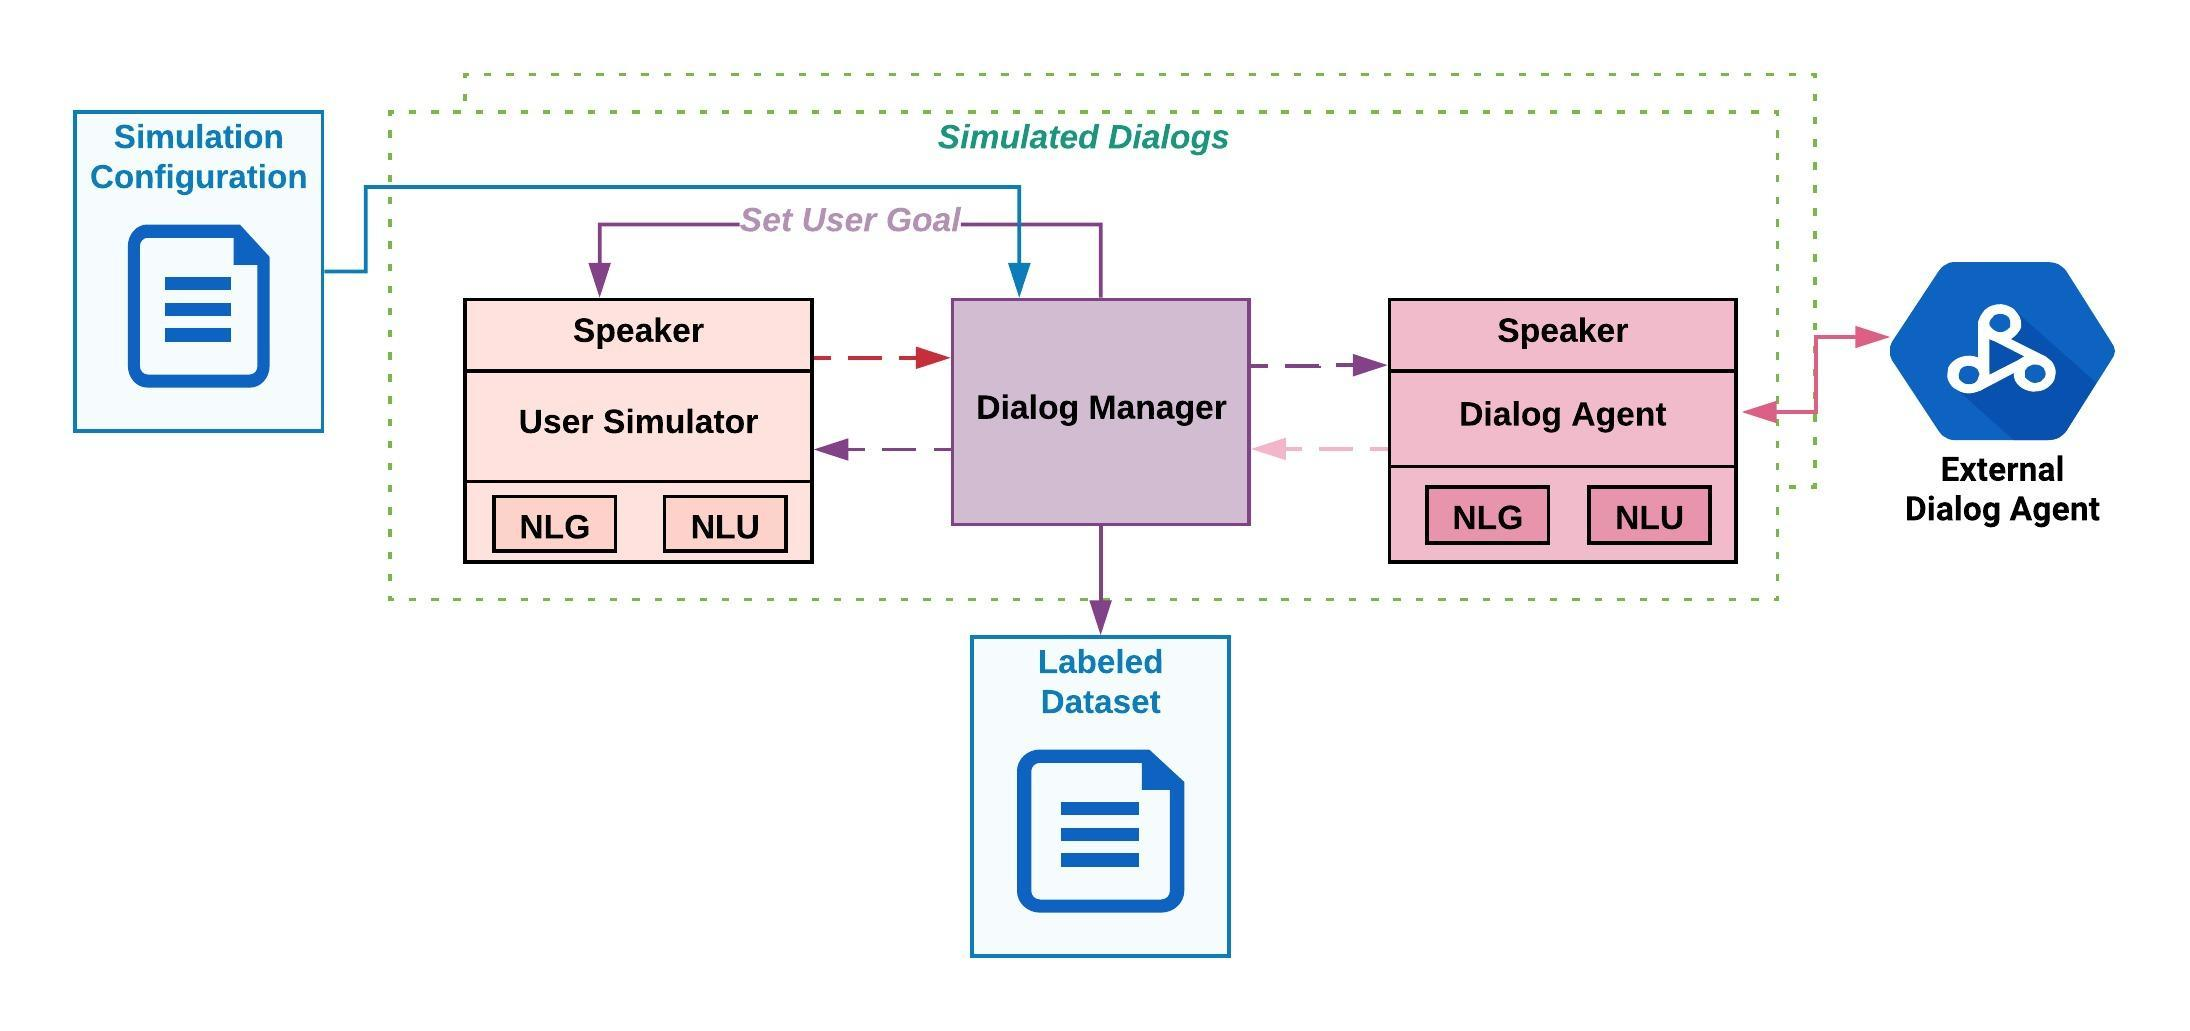
\includegraphics[width=\linewidth]{diagrams/socrates_diagram.jpeg}
	\caption{ Design of the Socrates Sim framework. }
\end{figure}

The Socrates Sim framework was designed to generalize to new domains and provide a consistent experience for dialog simulation and generation of labeled data. Figure \ref{fig:socrates_sim_framework} provides a high-level overview of the framework. The framework is simple. There are three key modules, the user simulator, the dialog agent, and the dialog manager. We assume that the user simulator and dialog agent have been implemented externally. In order to fit into the framework, they need to be integrated into implementations of the \textit{Speaker} abstract base class. The \textit{Speaker} abstract base class provides a set of APIs that allow for the user simulator and dialog agent to communicate with the framework in a standardized way. Once the classes are created, their locations are stored in a configuration file that is used by the dialog manager to load speakers and run simulations. The external configuration file as supports additional settings and figurations which allow rapid experimentation and make it easy to transition to new domains.

The framework needs to be modular so that it can be quickly adapted to support new dialog domains and experiments. Each major component of the framework is represented as a Python abstract base class. Both the user simulator and agent have the same base class (Speaker) and have their own internal nlg and nlu objects. The internal nlg and nlu objects are implementations of the \textit{NLG} and \textit{NLG} abstract base class. Additionally, communication between the speakers is standardized. Dialog actions, goals, and domain knowledge bases are all first-class objects. This is in stark contrast to the design choice of \cite{li_end_to_end}, where similar components are implemented as Python dictionaries. As first class objects, I can standardize the communication and management of these pieces and ensure more consistent behavior.

Another key distinction of Socrates Sim is that the framework is agnostic to how the dialog agent is implemented. By decoupling the agent from the dialog manager, the researcher is free to test out different agents without having to rewrite the entire simulation framework.  The dialog agent class provides a simple interface to allow external agents to plug into the simulation framework. This also frees up the dialog manager to provide other useful services like metrics, dialog analysis, and labeled data generation.

\subsection{Configuration First Design} 

We want to provide as much flexibility and freedom to the researcher and limit what is hard-coded. I follow the configuration-first approach leveraged in the development of AllenNLP, a deep learning for NLP tool developed at the Allen Institute for Artificial Intelligence. The objective of the approach is to separate out domain-specific logic from implementation details. The configuration file stores information about the domain and domain specific implementation choices. As a result, the implementation code can be written at a higher level and be more flexible and re-targetable. 

To support a configuration-driven approach, each configurable module will support the ingestion of a user-defined yaml or json file. For smaller configuration details, the user may prefer to use the yaml format which is more human readable. The yaml format is simple and has a very low learning curve. It follows a basic key-value pair paradigm, where keys have clear semantic meaning and values can be represented in a variety of data structures. 

\begin{figure}[h!]
	\begin{lstlisting}
	# Dialog Simulation settings
	simulation_rounds: 10
	max_turns: 8
	first_speaker: usersim
	simulation_output_path: data/simulated_dialogs/
	\end{lstlisting}
	\caption{Example yaml section.}
	\label{fig:ex_yaml}
\end{figure}

Socrates Sim is a command line tool. Once the researcher has set up the user simulator and dialog agent, they can invoke the dialog manager and run simulations with the command line. At the end of the simulation, the dialog manager will output performance metrics for the dialog agent and store the generated dialogs with annotations.

The remainder of the chapter will further describe in detail the different components of Socrates Sim.

\section{Dialog Domain and Domain Knowledge Base}
\label{sssec:dialog_domain}

\begin{figure}[h!]
	\centering
	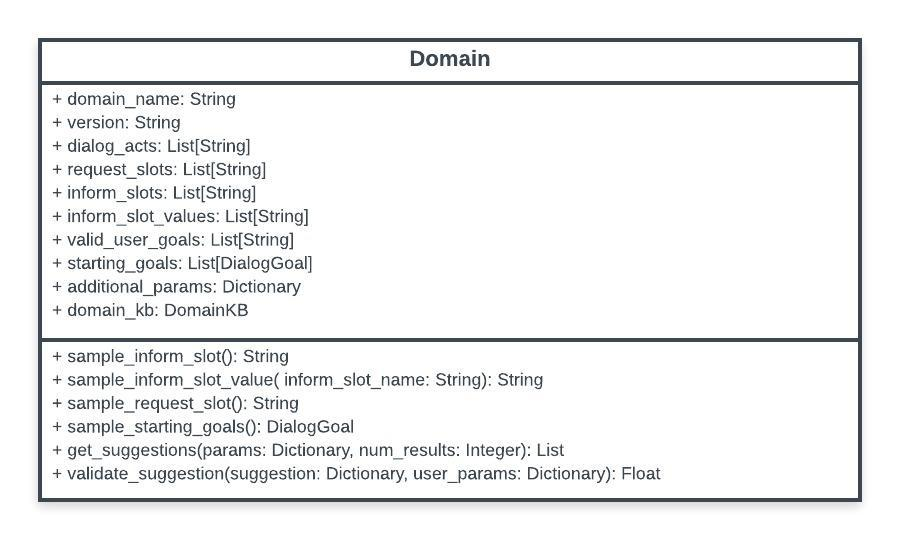
\includegraphics[scale=.9]{diagrams/domain_class.jpeg}
	\caption{ Dialog domain class. }
	\label{fig:domain_class}
\end{figure}

The domain class standardizes the collection and storage of information related to the domain of the services provided by the dialog agent. The domain class is initialized by a configuration file defined by the researcher and provides a set of APIs to access the various domain elements. The domain class consists of the following key properties: dialog acts, request slots, inform slots and inform slot values, valid user goals templates, sample starting goals list, and a domain knowledge base object.  Additionally, the following key API methods are made available: sample inform slots and inform slot values, sample request slots, get valid user goals, and get suggestions (from domain knowledge base) and validate suggestions. 

The primary consumer of the domain class is the dialog manager, which uses the domain information to generate new user goals or sample user goals from a preexisting list of starting goals. If the dialog manager is generating novel user goals, it will use the valid user goals template to create a new goal and sample the inform slots to generate the user's preferences for that goal. The domain object is also provided to the user simulator and dialog agent for use. 

The domain knowledge base (KB) is an abstract base class. Its purpose is to define a standardized way for a speaker to query and access the knowledge base. The primary purpose of the domain KB is to store all the suggestions that a dialog agent would make based on the various preferences of the user. The domain KB provides an interface with the following three methods; get suggestions, validate suggestions, and get the item. The researcher is free to use whichever back-end and implementation to resolve those three API calls. 

\begin{figure}[h!]
	\centering
	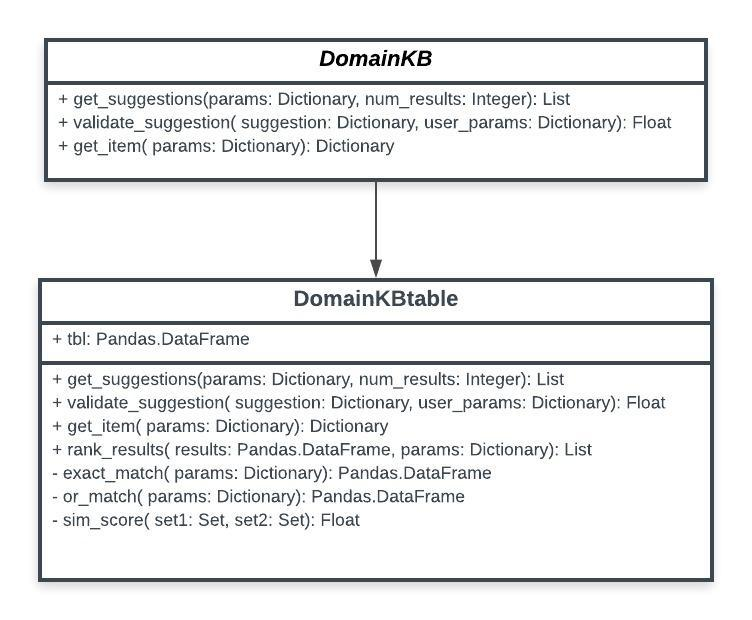
\includegraphics[scale=.8]{diagrams/domain_kb_class.jpeg}
	\caption{ Domain knowledge base abstract base class and implementation.  }
	\label{fig:domain_kb}
\end{figure}

For this thesis, \textit{DomainKBtable} is an implementation of the \textit{DomainKB} abstract base class. It loads tabular data from a csv file into a pandas data frame. The pandas data frame is a memory efficient data structure that supports querying and data manipulation. More details about the \textit{DomainKBtable} can be found in the implementation chapter. 

\section{Speaker Abstract Base Class}
\label{sssec:speaker}

The \textit{Speaker} abstract base class represents an actor that has the ability to speak and comprehend speech utterances. In our framework, both the user simulator and the dialog agent are represented by the same base speaker class. Both actors are conceptually identical in terms of functional behavior. They listen and comprehend speech utterances and respond in turn by speaking. Thus, both the user simulator and dialog agent can be represented in the same way to the dialog manager. In fact, the entire conversation round can be expressed in two lines (see Figure \ref{fig:conv_round}).

The speaker class has four basic functions (\textit{next, reset, get utterance, and parse utterance}) and three properties (\textit{nlg model, nlu model, and dialog status}). When the speaker is initialized, the natural language object and the natural language understanding object are passed to the constructor. We abstract away the implementation of how the speaker speaks and parses speech in order to maintain separation of concerns and also empower the researcher to be able to experiment with multiple techniques. 

The \textit{next} method is the primary driver for how the speaker behaves. For the dialog agent class, the next method functions as an API to the simulator. It is assumed that the dialog agent is external to the simulator. The researcher can define how the dialog agent will interact with the user simulator here. For the user simulator, the bulk of the logic will reside here. The \textit{get utterance} and \textit{parse utterances} methods are simply wrappers for the speaker's nlg and nlg objects. The primary parameter for next is the previous dialog action. 

\begin{figure}[h!]
	\centering
	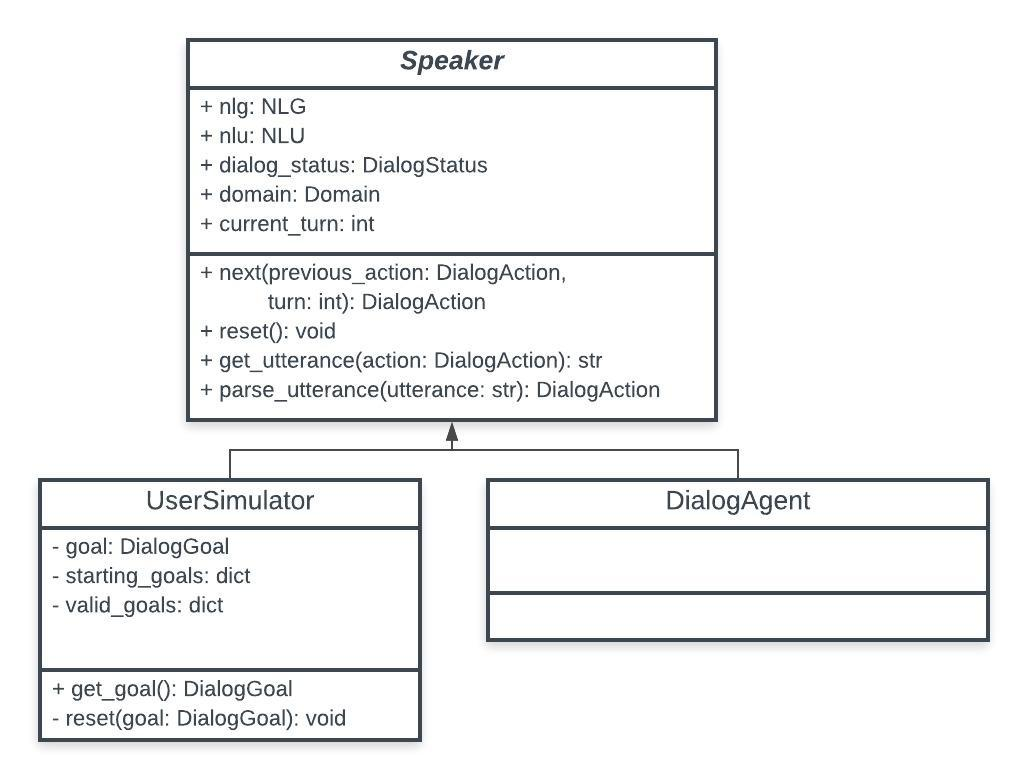
\includegraphics[width=\linewidth]{diagrams/speaker_classes.jpeg}
	\caption{ Speaker abstract base class and implementations.}
	\label{fig:speaker_class}
\end{figure}

\subsection{User Simulator}
The user simulator is responsible for imitating a real user and generating realistic speech utterances. Here we assume the user is an actor that is attempting to complete a task. For example, the user may want to travel to Japan and is attempting to book a flight there. That user could then interact with a travel agent chatbot in order to get assistance in identifying the appropriate flight and purchasing tickets. In order to model and represent a user, we will utilize the formalization of the hidden user agenda described in \cite{Schatzmann2009TheHA}.

One of the primary assumptions here is that the user has intentionally engaged with the dialog agent in order to complete their task. At the outset of the conversation, the user will have some specific goal in mind (order Indian food, book a flight to Japan, etc). The dialog agent will attempt to learn the user's goal by asking the user a set of clarifying questions. Schatzmann and Young introduce the idea of a hidden user agenda as a mechanism to represent the sequence of dialog acts and utterances a user will say in the context of that conversation. At each step of a task-completion dialog, the user is either responding to the dialog agent or initiating a new conversation direction. The user agenda provides an efficient way and formal structure to represent the pending set of dialog acts the user will communicate to the dialog agent.

The user agenda and user goal are first class objects and are described in further detail below. Additionally, we use the \textit{UserSimulator} class (see Figure \ref{fig:speaker_class}) as an implementation of the \textit{Speaker} abstract base class. This user simulator is required to be more transparent and accessible in a particular manner by the dialog manager. At the beginning of each round, the dialog manager generates a user goal and updates the user simulator with that goal. Additionally, at the end of each conversation round, the internal state of the user simulator's goal is extracted and stored in the dialog history that is being actively tracked by the dialog manager. As a result, the researcher must implement a get\_goal and override the reset method in addition to the interface methods defined in the \textit{Speaker} abstract base class. The dialog goal is formalized as a \textit{DialogGoal} object and more details about it can be found in section \ref{sec:dialog_goal}. 

\subsubsection{User Agenda} 
~ \\
\cite{Schatzmann2009TheHA} define the user agenda as a \textit{“[stack] structure of pending dialogue acts [which] serve as a convenient mechanisms for encoding the dialogue history and user’s ‘state of mind’”}. Formally, at any time t, the user is in a state s\textsubscript{u} and takes an action a\textsubscript{u},which transitions into an intermediate state s\lq\textsubscript{u}. During this intermediate state, the user will receive an action from the system (machine) am, which will transition dialog to next state s$''$ \textsubscript{u} and the cycle will reset. The result is a sequence of alternating turns between the user and system (i.e. s\textsubscript{u} $->$ a\textsubscript{u} $->$ s$'$\textsubscript{u} $->$ a\textsubscript{u} $->$ s$''$\textsubscript{u} $->$ \dots), which represents the conversation state over time t.

The user agenda is a stack-like structure which contains all pending user actions. User actions are actualized through popping the stack and the agenda is updated by pushing back onto the stack. A user action is a representation of the user’s intent, which will eventually be translated into a speech utterance. The stack may also contain other actions that will affect the user when popped. For example, the system can communicate a restaurant suggestion, which would fill one of the request slots with the restaurant name.  

At the start of the dialog, a new goal is randomly generated from the provided dialog domain. An accompanying agenda is then generated to represent the potential sequential of events. 

Below is an example of the sample user agenda that Schatzmann and Young provide in the context of a user asking the dialog system for a bar recommendation [6]. The states of the conversation are indexed by time t. Note, Schatzmann and Young use constraints C, which would be the equivalent of inform slots in our representation. In the first turn, the user simulator generates a set of constraints (bar serving beer in central) and goals (name, address, and phone for a bar that meets the constraints in C\textsubscript{0}). This set of inform and request slots are translated into a user action stored in A\textsubscript{0}. When the system initiates the conversation, the user simulator pops two inform actions which translate into the user utterance \textit{I’m looking for a nice bar serving beer}. When the system at t=1, responds \textit{Ok, a wine bar. What price range?}the agenda updated to include a new inform intent (inform(prange=cheap)). Also added is a negate action, as the user asked beer and not wine. 

\begin{figure}[h!]
	\centering
	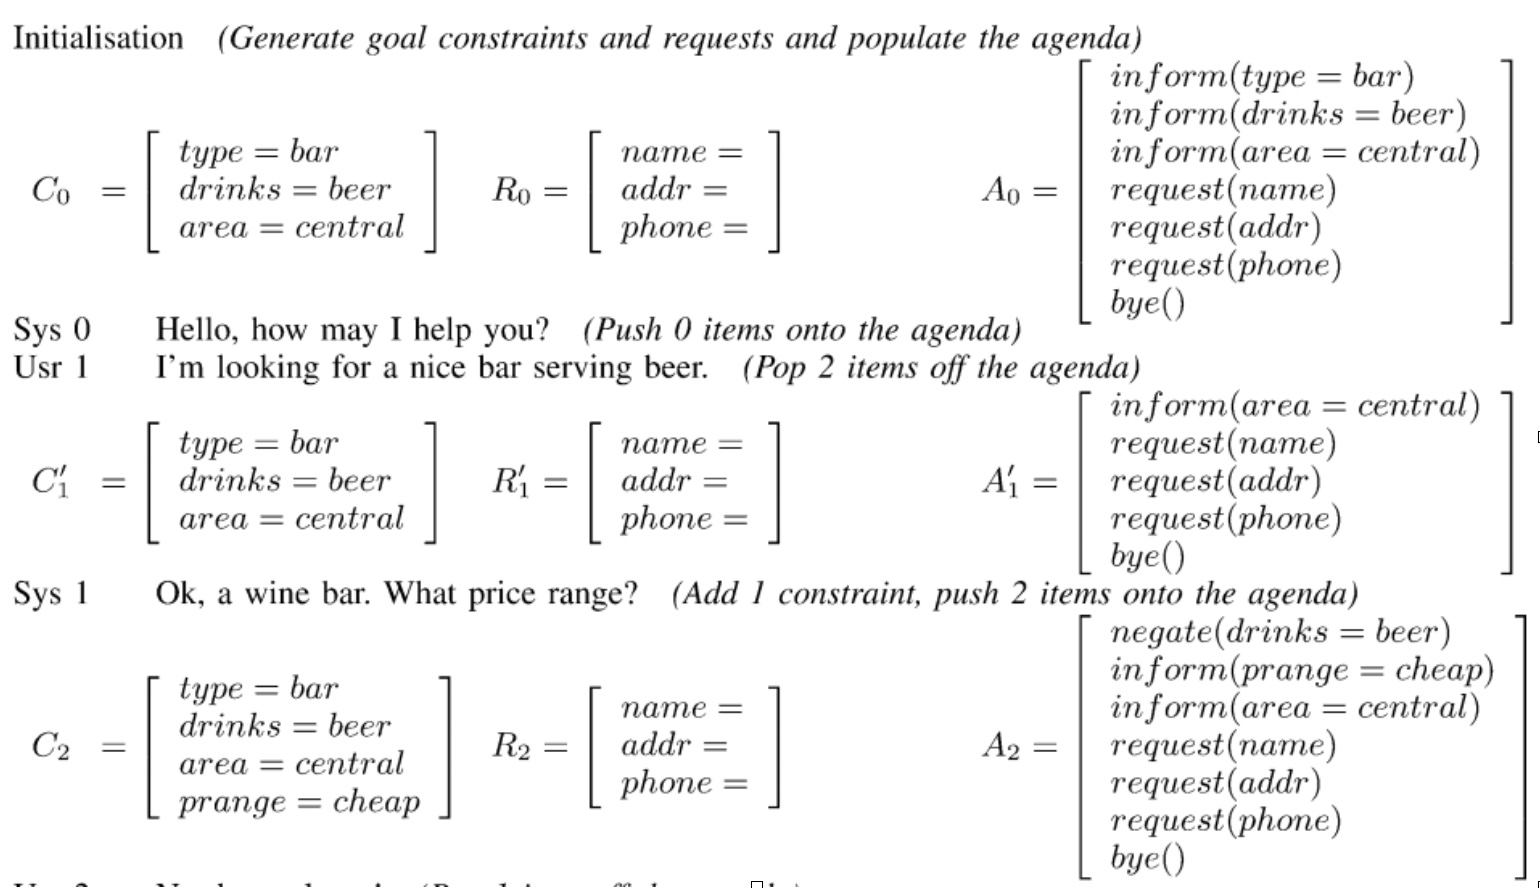
\includegraphics[scale=.25]{diagrams/ageda_ex2.jpeg}
	\caption{ Example of user agenda formulation from \cite{Schatzmann2009TheHA} }
	\label{fig:speaker_class}
\end{figure}

Over the course of the conversation, the agenda is updated, as are the request slots. The conversation ends at t=5 when bye() is popped and the agenda stack is empty. The conversation will then be evaluated based on how well the request slots were filled.

\subsection{Dialog Agent}
The framework assumes that the dialog agent is opaque and can only communicates with the framework through dialog action objects.Therefore the \textit{DialogAgent} class in Figure \ref{fig:speaker_class} serves more as a template for implementation. Implementing the four methods defined in the \textit{Speaker} abstract base class, allows for the dialog agent to communicate with the dialog manager. We explore the implementation details in Section \ref{sec:speake_interface} for the \textit{DialogAgent} class.

\section{Key Dialog Components}
In order to standardize communication, we have formalized the concepts of dialog action, dialog goal, and the nlu and nlg processes. In the sections below, we investigate them in further detail.

\subsection{Dialog Action}
\label{sssec:dialog_action}

\begin{figure}[h!]
	\centering
	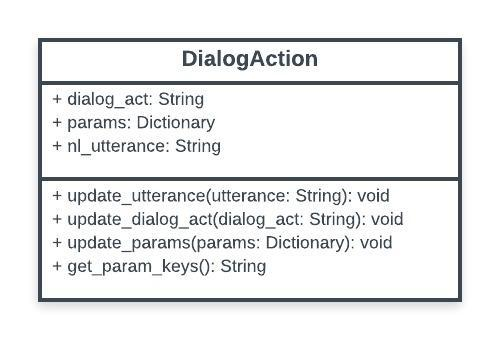
\includegraphics[scale=1]{diagrams/dialog_action.jpeg}
	\caption{ Dialog action class. }
	\label{fig:dialog_action_class}
\end{figure}

The fundamental unit of transaction for the simulator is the dialog action. It is an explicit semantic representation of the speech utterance that is machine readable. For example, I could represent the speech utterance, \textit{I'm looking for a Thai restaurant}, in the following way: \\
\textbf{original utterance}: \textit{I'm looking for a Thai restaurant}   \\
\textbf{dialog act}: \textit{request}\\ 
\textbf{constraints}: \textit{cuisine=Thai}\\

The \textit{DialogAction} object encodes information about a speech act in a standardized way. The dialog action consists of three key properties: the dialog act, a set of explicit dialog parameters or constraints, and corresponding unparsed speech utterance. I will next describe these properties in further detail. 

The unparsed speech utterance is just the natural language utterance that was spoken by the speaker One of the objectives of the user simulator is to generate speech utterances based on its internal agenda. The user simulator will use the dialog act and dialog parameters popped from the user agenda in order to generate a new utterance using its natural language generation model. If a speaker is hearing the utterance, then the utterance will need to be parsed and broken into a dialog action and set of parameters. 

The dialog act property is used to capture the intent of the speech act. Common dialog acts include: inform, request, confirm, negate, and affirm. The dialog act is necessary to provide context for the dialog parameters for both the natural language generation and language understanding use cases. For example, a set of dialog parameters like \textit{{cuisine=thai, area=north}} can be interpreted differently in the inform vs request context. In the request context, the speech utterance could be I\textit{'d like to find a Thai restaurant in the north part of town.} In contrast, those same dialog parameters could be part of a suggestion in the inform context. E.g. \textit{There is a great Thai restaurant in the north part of town}. Given the variability of dialog acts and intents, the space of possible dialog acts is defined by the researcher in the dialog domain configuration file. While this limits the possible interpretations of a speech act, a reduced dialog act space is beneficial to building effective task-completion dialog agents.  

The dialog parameters property encodes entities found in the speech utterance as key-value pairs and is used the communicate or elicit the user's preferences. The key captures the entity/constraint type (e.g. cuisine, area, address, etc), while the value is used to indicate the specific constraint or entity (e.g. Thai, north, 115 Way Street, etc). The parameter property is strictly typed as a Python dictionary and therefore all keys must be associated with a value. In the context of request speech acts, the null value is used to indicate the speaker wants to elicit more information the provided constraint type. For example, \textit{dialog\_act=request, params=\{address: NULL\}}, would be interpreted as a request for the address (e.g.\textit{What is the address?}). 

Initially, I used Python dictionaries and sets to represent the dialog parameters. However, this was sub-optimal for several reasons. First, it introduced variability and uncertainty. To capture the request parameters, I used Python sets, since the value was null and we just needed to pass along the constraints types. For all dialog actions, I had used explicit dictionaries as real values were passed along with the constraint types. However, downstream this required logic to check the class instance of the parameter variable being passed in. 

Given the dynamic nature of the dialogs being generated, the simulator was rather unstable and would randomly crash when a method expecting a dictionary received a set. By enforcing the Python dictionary type and setting null values, I was able to greatly improve stability and make debugging easier by standardizing the input into functions that consumed the \textit{DialogAction} object. 
\clearpage

\subsection{Dialog Goal}
\label{sec:dialog_goal}

The user goal captures explicitly the speaker's preferences and missing information they are trying to acquire. For example, take a user who wants to find an Indian restaurant in Central Square for dinner. We can decompose this goal into two distinct components. The first is the user's explicit preferences. In this example, their preferred cuisine is Indian. The second component is implicit and unknown to the user. They are looking for a restaurant or more specifically the name and presumably the restaurant's phone number and address. This information is unknown but can be broken down into discrete pieces of information the user will attempt to elicit from the dialog agent as a request for more information. 

\begin{figure}[h!]
	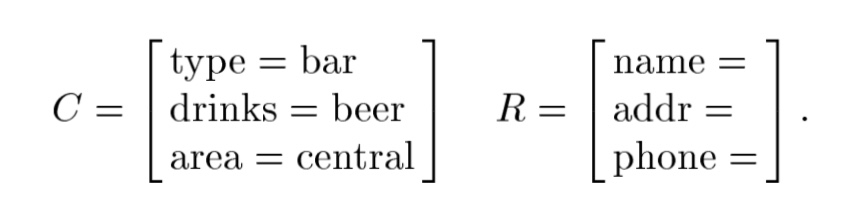
\includegraphics[scale=.35]{diagrams/schatzmann_goal_fig.jpeg}
	\caption{Example user goal. User wants the name, address and phone number of a cheap bar in central.  \cite{Schatzmann2009TheHA} }
	\label{fig:goals1}
\end{figure}

Formally, Schatzmann and Young defines the user goal \textit{G} as \textit{G = (C,R)}, where \textit{C} consists of constraints or the user's explicit preferences and \textit{R} represents the user's requests. The constraints and requests are explicitly represented as slot-value pairs. \ref{fig:goals1} below shows how one could represent the goal of a user looking for a bar. 

\begin{figure}[h!]
	\centering
	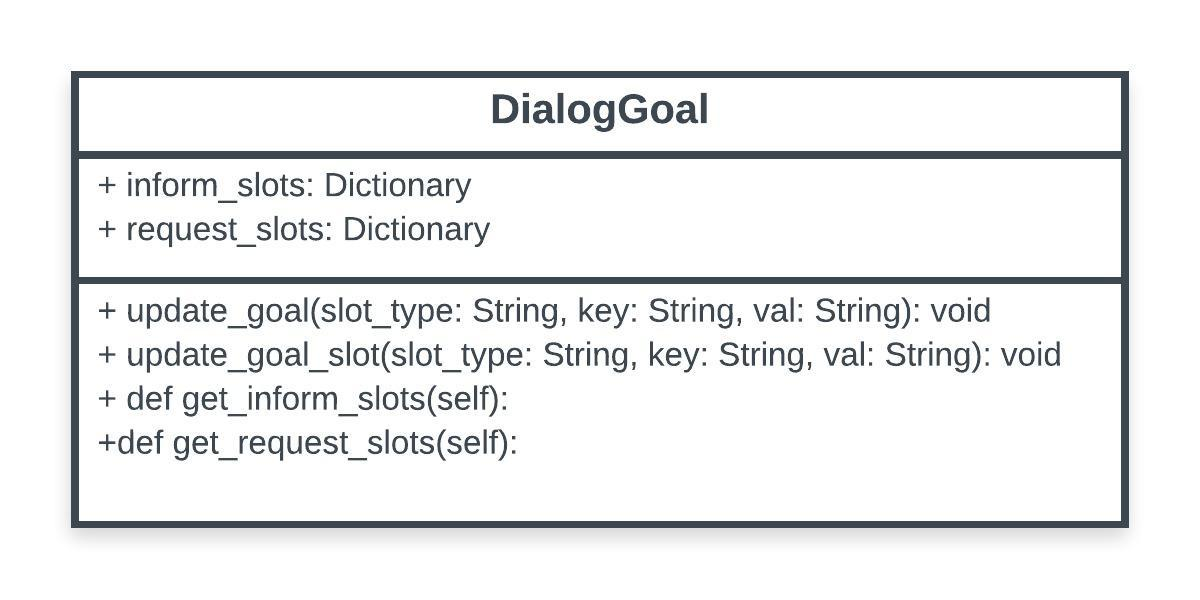
\includegraphics[scale=1]{diagrams/dialog_goal_class.jpeg}
	\caption{Dialog goal class.  }
	\label{fig:goal_class}
\end{figure}

The \textit{DialogGoal} class formalizes the Schatzmann and Young concept of the user goal. The concept of a goal abstractly turns out to be useful in also driving the dialog manager's simulations. We abstract the idea of the user goal and make it available to both the user simulator and dialog agent as a way to track the internal state of each speaker. 

For the user simulator, the goal defines the hidden set of preferences and information needs the user has. The goal object has two properties: inform slots and request slots. Both the inform and request slots are typed as Python dictionaries. The inform slots capture the user's preferences that they want to communicate to the dialog agent. A well-developed dialog agent should be able to elicit those preferences efficiently and ideally without needing to ask the user multiple times. The request slots capture the information user needs in order to complete their objective and task. At the start of the conversation, all the request slots values are set to null values. Over the course of the dialog, as the dialog agent responds the user simulator, the request slots may be updated with real values. A dialog is considered successful if all the request slots for the user simulator have been replaced by real values. The user simulator monitors the state of the request slots in it Goal object. If all the request slots are filled, the user simulator updates its internal dialog status to the complete state and signal to the dialog manager to end the conversation. 

In the first iteration, only the user simulator had the \textit{DialogGoal} object. But it made sense to allow the dialog agent to have access to its own \textit{DialogGoal} object. The rationale behind this was two-fold. First, it provides a useful mechanism to track the state of the dialog agent as well. Like the user, the dialog agent has its own set of goals, i.e. to elicit the information it needs to provide a meaningful suggestion or provide the specific service the user desires. The request slots in the dialog agent are complementary to the user's inform slots. The dialog agent can elicit the user's inform slot through a series of request speech acts and then execute its service. This leads us to the second value for the dialog agent, the \textit{DialogGoal} object provides a useful mechanism for training (especially in the reinforcement learning context). In failure cases, it signals to the researcher the information the dialog agent was ineffective in capturing. For reinforcement learning, a loss function can be developed that minimizes the open request slots in the agent's \textit{DialogGoal} at the end of each conversation when the agent renders its service. 


\subsection{Dialog Status}

The \textit{DialogStatus} is a Python enumerative object that encodes the internal state of the dialog for each speaker. Each speaker is responsible for setting its own dialog status. The valid states are not started, no outcome yet and finished. The dialog manager will probe each speaker for its dialog state. It the dialog manager learns that the state for any speaker is set to finished, the conversation will be ended. The user simulator sets its dialog status to finished when all the requests slots in it Goal object are filled. In contrast, the dialog agent may only set its state to finished after the user leaves the conversation. This way the agent does not prematurely exit the conversation before the user can complete their task. 

\clearpage

\subsection{NLG and NLU Abstract Base Class}


\begin{figure}[h!]
	\centering
	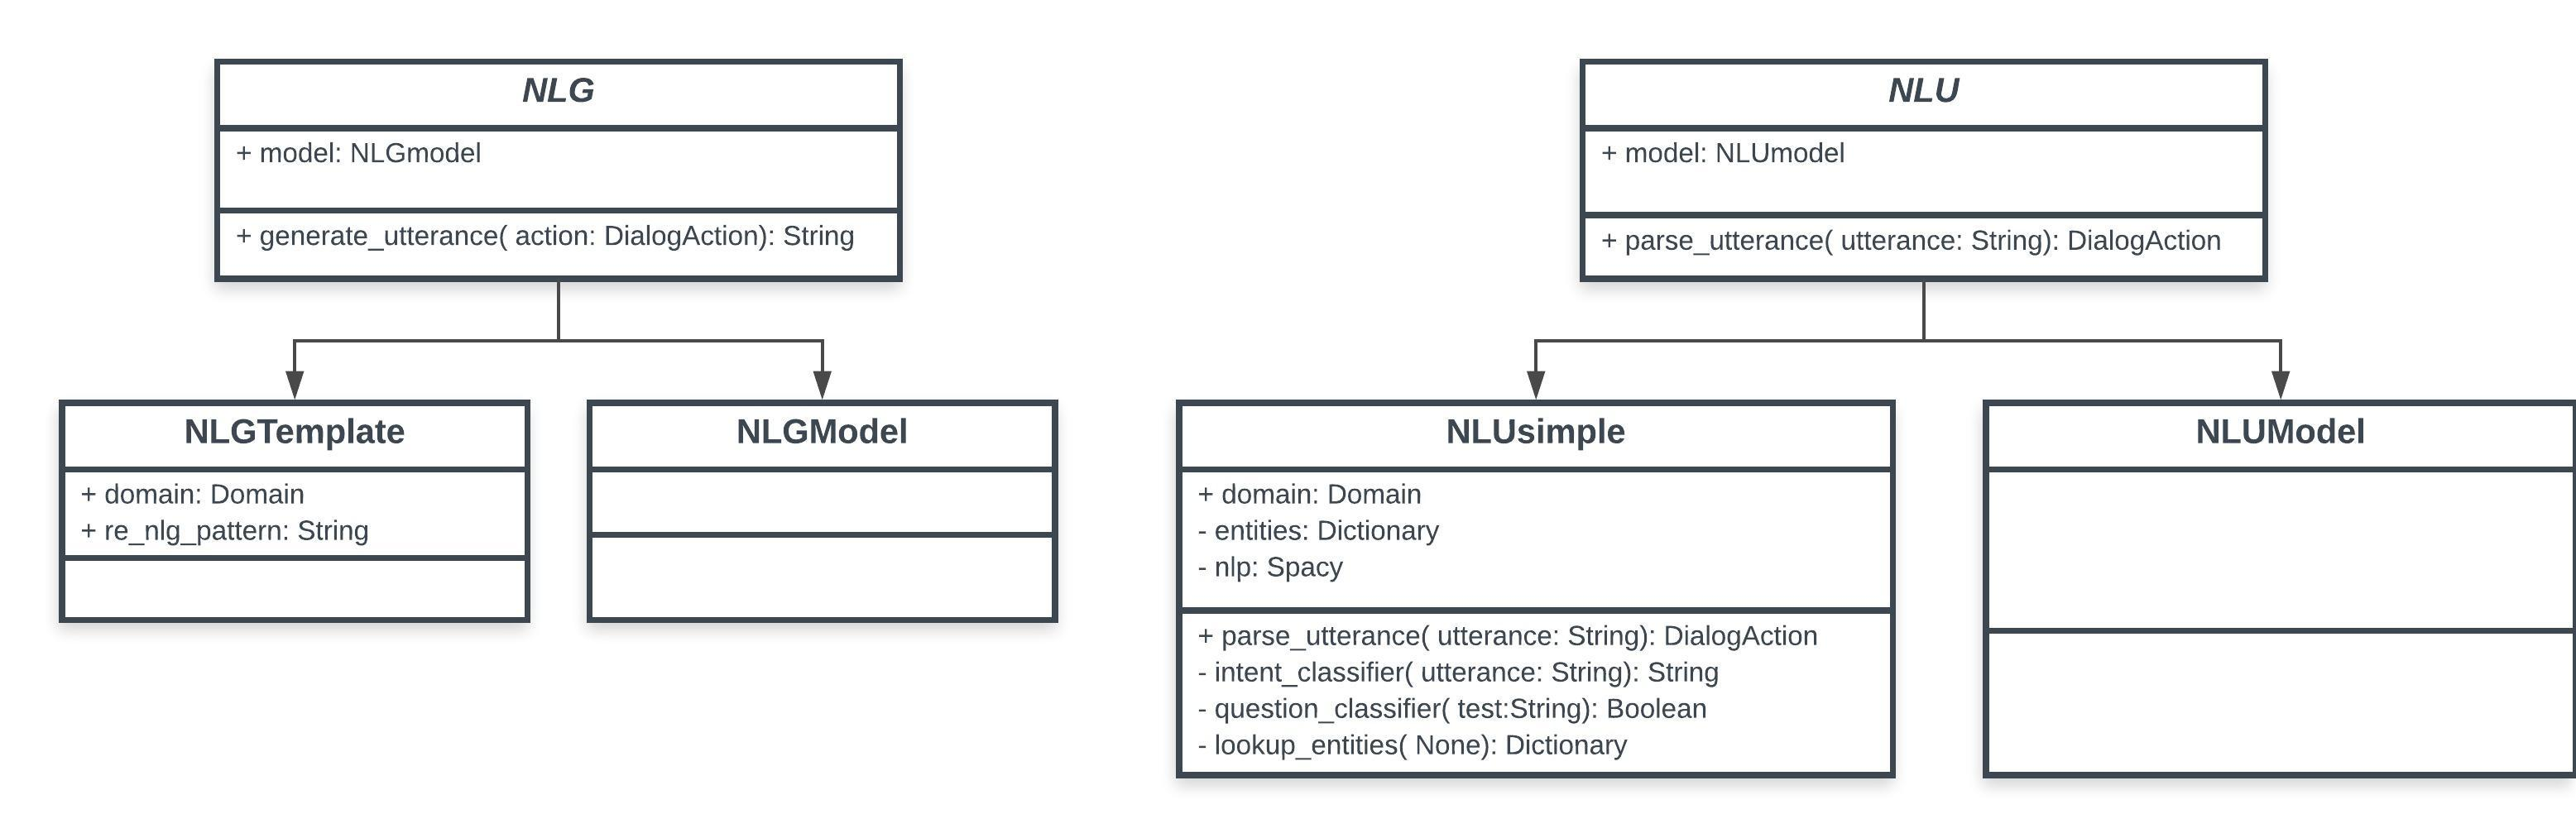
\includegraphics[ scale=.6]{diagrams/speaker_interface.jpeg}
	\caption{ NLU and NLG abstract base classes.}
	\label{fig:nlg_nlu}
\end{figure}

The NLU and NLG interface provides a common API for the parsing and generating speech utterances for each speaker. Both interfaces define a single public-facing API method: parse utterance and get utterance respectively. Parse utterance will take in a natural language speech utterance and return a \textit{DialogAction} object. Get utterance takes in a dialog action and returns a natural language speech utterance.

The researcher has flexibility in setting up the NLU and NLG back-ends. In the implementation section, we will further detail the simple rules-based approach and neural machine translation implementations for both the nlg and nlu back-ends. 

Upon initialization, the speaker class will set an internal nlg and nlu object. The speaker's\textit{ get\_utterance } and \textit{parse\_utterance} will directly call the correspond methods in the nlg and nlu object. This way the dialog manager does not need to know the internals of each speaker's nlg and nlu objects. 

Nlu and nlg are open problem space and there are no universal solutions. In abstracting the nlu and nlg interfaces, the researcher has more flexibility in training and experimenting with their dialog agent. Since the user simulator will always return the machine-readable dialog action with the generated speech utterance, the researcher has the ability to train the nlu for their dialog agent to support more robust NLU use cases. 

\section{Dialog  Manager}

\begin{figure}[h!]
	\centering
	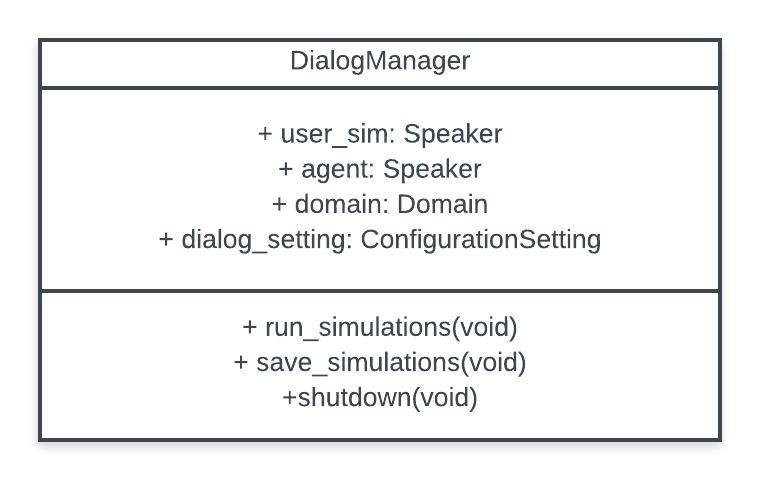
\includegraphics[ scale=1]{diagrams/dialog_manager.jpeg}
	\caption{ Dialog manager class. }
	\label{fig:dialog_manager}
\end{figure}

The dialog manager is the primary engine of the simulation framework. Its responsibilities include loading the dialog domain, setting up user simulator and dialog agent, running the simulations, and performing post-simulation metrics. The dialog manager does not need to modify by the researcher and is set up to implement the researcher's simulations via a configuration file. The configuration file is translated into a configuration object by the command line tool and sent to the dialog manager. In the configuration file, the user specifies the following:
\begin{itemize}
	\item user simulator class
	\item dialog agent class
	\item dialog domain representation
	\item domain knowledge base class
	\item simulation settings 
\end{itemize}

The dialog manager uses Python dynamic loading capabilities to import the end user custom classes for the user simulator, dialog agent, and domain knowledge base. Once these are loaded into memory, the simulator runs the simulations. Figure 
\ref{fig:dialog_model} shows at a high level what the dialog model looks like. 
\begin{figure}[h!]
	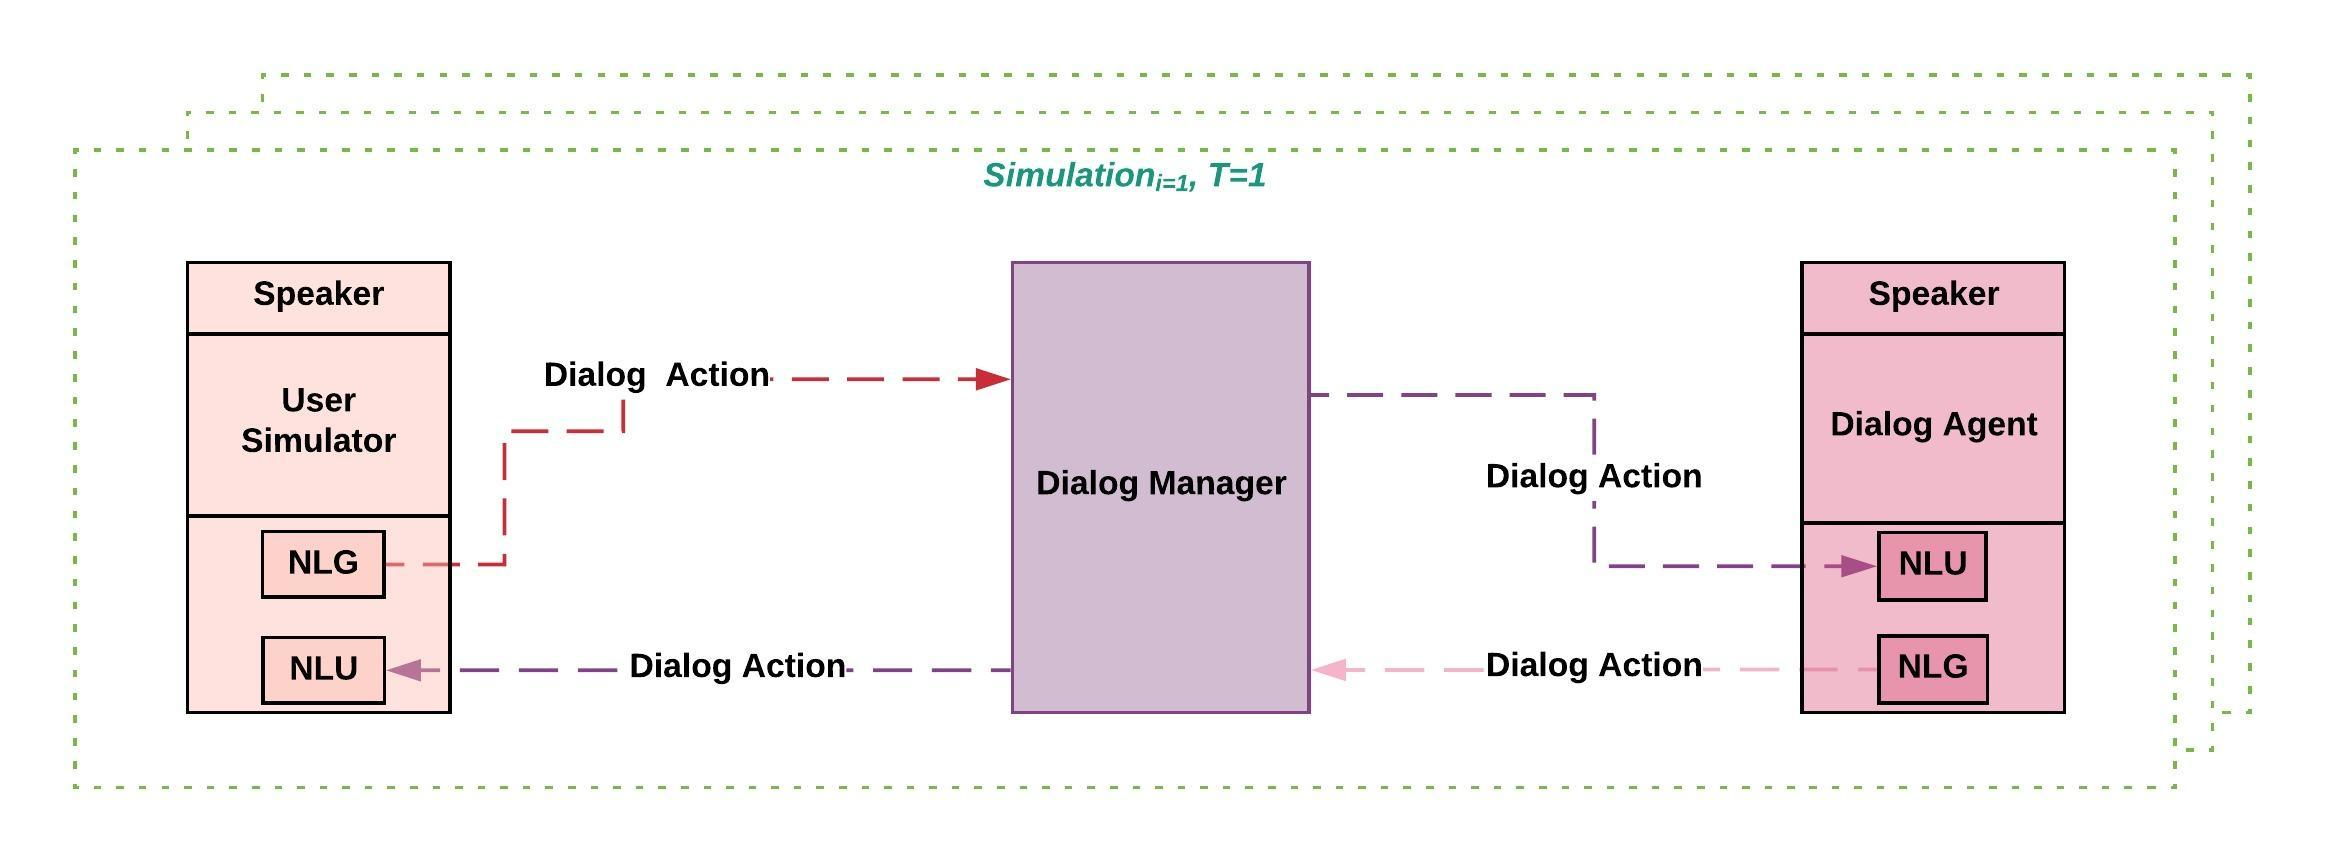
\includegraphics[width=\linewidth]{diagrams/dialog_model.jpeg}
	\caption{ Dialog model overview. }
	\label{fig:dialog_model}
\end{figure}

The dialog manager follows a basic pattern when running the simulation. It first generates a user goal, which will drive the user's hidden agenda and behavior. Next, it resets the user simulator with the newly generated goal and calls the dialog agent to reset itself. Once both speakers are ready to interact, the simulation is initiated. The logic for conversation is quite straightforward. The speaker class has the next method, which takes in dialog action and returns a response dialog action. The logic for the speakers to communicate with each other can be expressed in two line (see \ref{fig:conv_round}. The dialog action object standardizes how the speakers talk to each other and detail can found below.  

Finally, in order to simulate a real user, the researcher can set configure the user simulator to be corrupted in different ways. The user can change their minds and have a new preference generated from the dialog domain. To simulate faulty technical issues, the user may randomly exit the conversation. And finally, the user's goals can be corrupted resulting in an indiscernible signal from the user as to whether their goals were met or not. All these corruption are specified by the researcher with a probability value, which represents the likelihood the user simulator will act aberrantly. This behavior will 
help generate more diverse data by providing negative examples.

\begin{figure}[h!]
	\label{fig:conv_round}
	\begin{lstlisting}
	# Assuming user speaks first 
	# 1. User Simulator takes turn and speaks
	user_action = user_simulator.next(previous_agent_action, turn_number)
	# 2. Agent takes turn and responds to user 
	agent_action = agent.next(previous_user_action, turn_number)
	\end{lstlisting}
	\caption{Pseudo code for conversation round.}
\end{figure}

Once all the simulations are run, the dialog simulator will run performance metrics to evaluate the efficacy of the dialog agent. If the user simulator was able to fill all the request slots in their hidden goal, the dialog is marked as successful. The researcher will be informed the average success rate of the dialog agent and can also see the round level evaluations in the generated dataset. After all simulations have been run, the dialog manager will serialize the output (if specified by the researcher) and exit. The goal of the output file is to provide quality annotated data that can be used as training data for supervised learning or reinforcement learning based dialog agent. 



%%% Local Variables: 
%%% mode: latex
%%% TeX-master: "main"
%%% End: 



\chapter{Implementation}
\label{chap:implementation}

\section{Overview}

In this chapter, we will the deployment of the Socrates framework in two domains, restaurant recommendation and movie tickets. We will demonstrate how the framework's robustness, modularity, and ability to be re-targeted across new domains. For each domain, we describe the setup configurations used, implementation details for the user simulator, dialog agent, and the various constituent models implementations like natural language generation and knowledge base querying. Note the full implementation code can be found in the appendix. We will focus on the strategies deployed and in particular the flexibility of the framework to handle different implementations.

\section{Restaurant Recommendations}

\subsection{Overview}

The restaurant recommendation domain focuses on developing a chat-bot service that makes restaurant recommendations. The objective of the Socrates simulator is to produce a set of simulated conversations between the user simulator and Restaurant Recommender dialog agent. The dialog agent will attempt to elicit as much information about the user's preferences and then attempt to provide a useful recommendation. In this task completion exercise, both the user and the dialog agent can take the first turn. 

As mentioned in the Design chapter, the framework is driven by configuration files. The researcher can easily modify and run different experiments through updated a human readable yaml file or a programmatically generated json file. For this use case, four configuration files are created to capture the following information:
\begin{itemize}
	\item Simulation settings: contains all the details around simulation criteria (e.g. number of rounds, first speaker, save setting, etc) as well the configuration details for dialog domain, user simulator and dialog agent. 
	\item Dialog domain: describes the dialog action space, inform and request slots, and specifies valid user goals templates.
	\item NLG templates for user simulator and agent: a rules based template to generate natural language utterances 
\end{itemize}
Additionally, we created custom modules to implement the user simulator and dialog agent for an end-to-end dialog simulation. 

We used the Dialog State Tracking Challenge 2 (DSTC2) restaurant data and service as a model for our use case. The DSTC2 is research challenge put together by the University of Oxford and Microsoft to advance dialog research. For DSTC2, the goal was track the state of multi-stage conversations between real humans and a expert restaurant recommender service. The restaurant recommender service would provide recommendations based off the following user preferences: cuisine, area, and price range. DSTC2 also provided a rich and deep set of training data that allowed to model both neural network based approaches for NLG and NLU, as well as rule based approaches. 

Below we will describe our strategy for developing the user simulator and dialog agent using the Socrates Simulator Framework and implementation choices for their constituent parts. 

\subsection{Domain}

\begin{figure}[h!]
	\caption{ Restaurant Dialog Domain}
	\label{fig:restaurant_domain}
	\begin{lstlisting}
	# Dialog Action Space
	dialog_acts: [ inform, confirm, affirm, request, 
			negate, greetings, bye]
	
	# Request Slots
	request_slots: [ address, area, cuisine, 
			 phone, pricerange, postcode, name ]
	
	# Inform slots
	inform_slots: [ cuisine, pricerange, name, area ]
	
	# Valid User Goals Temaplates
	valid_user_goals:
	- [ name ]                    # User wants restaurant name
	- [ name, address ]           # User wants name and address
	- [ name, address, phone ]    # User wants name, address, and phone
	- [ name, phone ]             # Use wants name and phone
	\end{lstlisting}
\end{figure}
The first thing we setup is the dialog domain configuration file. This file is used to generate a domain object that will be used by both the user simulator and the dialog agent. For restaurant recommendations, we used dialog domain described in the DSTC2 ontology. The figure above details the s dialog action space, and the different inform and request slot types. The dialog domain was expressed as a yaml file, where each key captured the salient attributes of the domain. 

One important feature of this file is the valid user goals templates section. It specifies the valid types of goals a user may have when engaging the dialog agent. The user simulator will use it generate random goals that can explore the preference space and test the robustness of the agent. 

Note, the figure above does not include the all the possible inform and request slot values. Please see the [appendix ref] for the full configuration file.  

\subsection{Domain Knowledge Base }

The knowledge base for this use case is csv with various restaurants from the Cambridge area. Each row represents a unique restaurant and the column values capture the restaurant's cuisine, price range, area, phone number, and address. The data was scraped by Yelp. For the scraping script, see the appendix. The restaurants list was loaded as DomainKBtable object. The DomainKBtable loads the csv files as in memory pandas dataframes and provides a a set of methods for querying. 

\subsection{Natural Language Understanding Implementations}

The goal of NLU implementation is to parse a natural language utterance into a DialogAction object. The parsed dialog action contains the intent of the utterance, i.e. the dialog act, and any entity / entity types, i.e. the dialog parameters, which are contained in the utterance. A rules based model and neural model were implemented to demonstrate the different models a researcher can use to support the natural language understanding. 

\subsubsection{Rules Based NLU}

For the rules based approach, our parser has two part strategy. The first is to classify the intent of the utterance and map it to a dialog act. The second to is run an entity extraction pass and attempt to extract the entities contained in the utterance and map them to inform slot types. 

The algorithm for the intent classification consists of two parts. The first is running the utterance through a question classifier ( implemented from \cite{chewning_lord_yarvis_2015} ). If the utterance is a question, we classify it as a request dialog act. Otherwise run though a set of regular expression matches and return the corresponding dialog acts ( see \ref{fig:intent_clf} ). Given the wide range of potential string matches for inform, we use that as the default dialog act. 

\begin{figure}[h!]
	\caption{ Intent Classifier Algorithm}
	\label{fig:intent_clf}
	\begin{lstlisting}
	Classify Intent
		input: natural languge utterance
		
		IF input is a question:
			return 'request'
		ELSE IF input contains [you, you want, right?]:
			return 'confirm'
		ELSE IF input contains [yes, yeah, yup, correct, right]]:
			return 'affirm'
		ELSE IF input contains [no, nope, wrong, incorrect]:
			return 'negate'
		ELSE IF input contains [hi, hello]:
			return 'greetings'
		ELSE IF input contains [bye, goodbye, thanks, thank you]:
			return 'bye'
		ELSE
			return "inform"
	\end{lstlisting}
\end{figure}

After the intent is classified, we then check to see if any entities are found in the utterance that can be mapped to entity types. To achieve this, we first lookup all the slot values defined in the domain object. Next, we create a reverse map dictionary, where each unique slot value ( i.e. the entity ) is mapped to a slot type (e.g. cuisine or price range ). The NLU parser then tokenizes the utterance into set a of word trigrams and check if a slot type exists for the token in the reverse map. All positive matches are added to the dialog params list in the DialogAction object. Finally, the parse utterance will return a DialogAction object with parsed dialog act and a list of dialog parameters. 

\subsubsection{Neural Model for NLU}

We also implemented a simple neural machine translation model for our NLU module. 

The DSTC2 provides a large labeled dataset of conversations between human users and an human expert posing as the dialog agent. Between the train and development set were about 2000 annotated calls. All speech utterances ( between the human and agent ) were parsed and annotated. To train the NMT model, we extracted out all utterances and the corresponding parses ( expressed as json string objects ). The model was trained over X epochs and released.

SERT NMT model diagram.



\subsection{Natural Language Generation Implementations}

The objective of the NLG module is to generate a natural language utterance, provided a dialog action. For the restaurant recommendation use case, we implemented both a template based model and a neural model. 

\subsubsection{Template  Based Model}

The template model is defined by a yaml file (see figure \ref{fig:res_nlg}). The nlg template is loaded into memory as a nested python dictionary. The first layer of keys are indexed by the dialog acts ( e.g. request, inform, etc), and the corresponding values are dictionaries indexed by specific slot types. In the case where there are the are no slot types ( e.g. affirm ), the default value is used. The natural language templates are stored in lists at the values for the slot types.

\begin{figure}[h!]
	\caption{ Example NLG template for User Simulator }
	\label{fig:res_nlg}
	\begin{lstlisting}
	 affirm:
		default: [ "Yes.", "Yup.", "Yes, that's right." ]
	 greetings:
		default: [ "Hi, I'm looking for a restaurant.",
			   "Hi! Can you help me find a restaurant?" ]
	 inform:
		cuisine: [ "I'd like find a restaurant that serves $CUISINE.",
			   "I'm looking for $CUISINE food.",
			   "I want to eat $CUISINE food." ]
		pricerange: [ "I'm looking for a $PRICERANGE priced restaurant.",
			      "Looking $PRICERANGE priced food." ]	
	\end{lstlisting}
\end{figure}

The logic then is straight forward to generating a natural language utterance. The get utterance method in simulator will be passed a dialog action object which contains the dialog act and a list dialog parameters. We first look up the dialog act in the nlg template dictionary. Next we look up the slot values ( if any ) for the specific language templates. The slot values are passed in the dialog params property of the DialogAction object. Additionally, language templates that have multiples slot types, are indexed by combination of the slot types into a single string. We take the slot types, lower case them, arrange them by alphabetical order, and concatenate them together with comma separator into a single string. For example, "I want \$PRICE \$CUISINE" would be indexed by the string "cuisine,price". Finally, we randomly sample the list from the list of potential language template, substitute slot values, and return a generated natural language utterance. 


\subsection{Neural Model for NLU}

We also implemented a simple neural machine translation model for our NLU module. 

The DSTC2 provides a large labeled dataset of conversations between human users and an human expert posing as the dialog agent. Between the train and development set were about 2000 annotated calls. All speech utterances ( between the human and agent ) were parsed and annotated. To train the NMT model, we extracted out all utterances and the corresponding parses ( expressed as json string objects ). The model was trained over X epochs and released.

SERT NMT model diagram.


\subsection{User Simulator}

We designed a rule based user simulator given the simplicity of the dialog domain. In this use case, the user has a set of hidden preferences and is looking get name of a restaurant that satisfies those preferences from the dialog agent. Additionally, the user may also want to get some the restaurant's phone number and address.

At the start of each dialog round, the user simulator will be provided a goal from the Dialog Manager. For demonstration purposes we defined both an explicit set of user goals  and valid goal template for random goal generation The figure below shows what a sample goal would look like. 

\begin{figure}[h!]
	\caption{ Example User Goal. User is seeking the name and phone number of a cheap Chinese restaurant}
	\label{fig:ex_user_goal}
	\begin{lstlisting}
	inform_slots:
		cuisine: "chinese"
		pricerange: "cheap"
	request_slots:
		name: "UNK"
		phone: "UNK"	
	\end{lstlisting}
\end{figure}

The rules simulator we designed is a separate python module that will be dynamically loaded by the Dialog Manager at simulation time. The rules simulator class inherits the base UserSimulator class, which in turn is a subclass of Speaker. The rules simulator will implement two key public methods defined by the Speaker, \textit{next} and \textit{get utterance}. From the dialog managers point of view, what the rule simulator does under the hood is completely hidden. The \textit{next} method takes in the opposing speakers speech utterance 

The user agenda, which captures what the user simulator will communicate to the dialog agent, is simply the concatenation of the inform and request slot lists stored in the user goal. Functionally the user agenda is a stack of pending dialog acts that user will say over the course of the conversation. All key-value pairs captured in the corresponding inform and request slot lists are mapped to inform and request dialog acts. Over the course of the dialog, the top item at the stack, which gets popped, contains that dialog action for what the user simulator will do next. That action would be passed the the simulator's internal natural language generation module to generate a natural language utterance. 

 For memory efficiency, we do not actually implement the agenda, as the information already exists in user goal. Instead we pop directly from the inform slots list or defer the action generated by the next method for responses to the dialog agent. We keep track of state of conversation by check how many of the request slots have been filled with real values. The rules simulator runs sequentially through the request slots at the end of each conversation and updates its internal DialogStatus enum object. The logic for how the user simulator responds to incoming speech acts from the dialog agent is handled by the \textit{next} method.
 
 \begin{figure}[h!]
 	\caption{ Internal logic for the rules simulator. }
 	\label{fig:ex_user_goal}
 	\begin{lstlisting}
 	response_router = { "greetings": respond_general,
 	"inform": respond_to_suggestion,
 	"random_inform": respond_random_inform,
 	"request": respond_request,
 	"confirm": respond_confirm,
 	"bye": respond_general}
 	
 	\end{lstlisting}
 \end{figure}

The \textit{next} is the driver of the rules simulator. It first will first attempt to parse the agents incoming dialog action and then respond to it using an internal dispatch tree. The internal logic of the \textit{next} method is a simple dispatch dictionary, where incoming dialog acts are mapped to resolver functions. Each response function has the same method signature, which is to take in a DialogAction object and return back a DialogAction that represents the user's response to dialog agent. The dialog agent's dialog action space is limited. The agent will respond with one of the following dialog acts:
\begin{itemize}
	\item greetings: the agent will greet the user and list it's services
	\item request: the agent will ask a probing question to elicit the users preferences
	\item inform: the agent will supply the user with information (usually tied to the user request request slots)
	\item confirm: the agent will ask the user to confirm if it understood the user's intent 
	\item bye: the agent will end the conversation  
\end{itemize}

The implementation of how the resolvers for the greetings, bye, and confirm responses are straight forward. The code implementation can be found in the appendix. For greetings resolver, if the rules simulator is the first speaker, it will invoke the random inform method one or several inform slots, which will be translated into an inform speech act. Otherwise, it handle the agent dialog action with the dispatch dictionary. 

The resolver for responding to the agents request actions is a bit more involved. The simulator will looked at the parsed request slots types the agent is asking about and attempt to find corresponding inform slots in it goal object. For example, if the dialog agent asks "What cuisine do you prefer?", the simulator will look up cuisine in its internal goal and return the answer Chinese (i.e based on the goal in \ref{fig:ex_user_goal}). In the case where requested slot type is not found in the user's inform preferences, the simulator will respond with either "I don't know" or "I don't care". This null response can be configured in the simulation configuration file, where the response either set to one of those two options or randomly chosen. Additionally, to simulate a realistic user, at configuration time, the researcher can also set the probability with which the simulator will "lie" or "change its mind" about its preferences. In those cases, the simulator will randomly sample the provided slot values in the dialog domain object and return a different slot value. 

If rules simulator has exhausted the informing the dialog agent of all its preferences, the simulator will then pop values from its request slots list and ask for a recommendation. If the dialog agent sent an inform action, the inform resolver method would update the request slot with new provided information. So for example, if the dialog agent made the suggestion, "Check out Golden Dynasty", the "UNK" value in \ref{fig:ex_user_goal} would be replaced by "Golden Dynasty". If all the "UNK" values in the request slots were filled with real values, the user simulator would update its internal status to complete and issue the bye action. 

As described above, the nlu and nlg models were set by the researcher in the simulation configuration file. By inheriting the UserSimulator class, the get utterance and parse utterance methods are also inherited and available to the researcher. Both method essentially call the corresponding methods in nlg and nlu objects. 

\subsection{Dialog Agent}

The restaurant agent was developed to illustrate how to incorporate an external dialog agent into the simulation framework. Since we do not have an existing restaurant recommendation agent, we developed a simple rule based agent. The goal of the agent is to capture all the user's preferences and then make a suggestion from its knowledge base of Cambridge restaurants. Like the user simulator, the public facing methods the dialog manager interacts with are \textit{next} and \textit{get utterance}. 

For the restaurant agent, we follow a simple rules approach. The agent expects to interact with the following dialog acts: greetings, affirm, negate, request, inform, bye. In situations where the agent encounters an unknown dialog act, it will repeat its last dialog act. At the beginning of conversation round, dialog agent internally resets its goal ( \ref{fig:ex_res_agent_goal} ). 

  \begin{figure}[h!]
 	\caption{ Restaurant Agent Goal }
 	\label{fig:ex_res_agent_goal}
 	\begin{lstlisting}
 	inform_slots: None
 	request_slots:
 		cuisine: UNK
 		area: UNK
 		pricerange: UNK 	
 	\end{lstlisting}
 \end{figure}

If restaurant agent goes first, it issues a greetings action. If the agent is not responding to user, it will sequentially pop one item from it request slots and issue a request dialog act. Once the restaurant agent has collected information from the user, it will attempt to make a suggestion from the knowledge base stored in the domain object. This is accomplished by calling the get suggestion method provided by the domain object.

\section{Movie Tickets}

\subsection{Overview}
The goal of the Movie Booking agent is help the end user purchase movie tickets. A similar domain agent was developed for the \cite{li_usersim} paper. Unfortunately, I was unable to use their agent and domain knowledge base in the context of the Socrates User Simulator. Much of their data was crowd sourced from Amazon Mechanical Turk and their use cases were a bit convoluted. There was a confusing overlap between the dialog action space for the user and agent which resulted in the user simulator making unrealistic utterances and dialog acts. There was a high ratio of nose and data quality issues which would have made it difficult to replicate.  

Drawing inspiration from their use case, the agent we developed is a bit more refined and modeled after something you would see on a movie booking site like Fandango. The agent will help identify movies for the user based on user preferences and also collect the user's payment details if the user choses to book a ticket. As the goal for this implementation is mainly to demonstrate the end to end dialog simulation framework and the user simulator, we did not implement an actual reservation database, a payment processing system, and a large move show times catalog. There are stubs for where the dialog agent would theoretically consult external resources in the aiding the user. We focus below on the the implementation details for the user simulator and domain modeling exercise.  

\subsection{Domain}

 \begin{figure}[h!]
	\caption{ Restaurant Agent Goal }
	\label{fig:ex_res_agent_goal}
	\begin{lstlisting}
	# Domain Information
	domain_name: movie
	version: 1.0
	
	# Dialog Acts
	dialog_acts: [ inform, confirm, affirm, request, negate, greeting, bye ]
	
	# Inform slots
	inform_slots: [ city, date, movie, rating, genre, 
	theater, times, zip, no_tickets ]
	
	# Request Slots
	request_slots: [ address, city, date, movie, rating, stars,
	state, theater, times, zip, genre, no_tickets, showtime ]
	
	# Required slots
	required_inform_slots: [ no_tickets, date, cc_number, cc_exp,
	cc_zip, cc_type, ccv ]
	
	# Valid User Goals
	valid_user_goals:
	- [ tickets_booked, movie, theater, showtime, address ]
	- [ tickets_booked, movie, showtime ]
	
	# Random integer contraints
	RAND_INTEGER_RANGE: [ 1, 10 ]
	\end{lstlisting}
\end{figure}

For the movie domain, we first set up the domain configuration file. This file is used to generate the domain object that will be used by both the user simulator and dialog agent. The inform and request slots reflect information that will be communicated and captured specifically for the movie book use case. The user will haves preferences that include desired movie genre, minimum movie rating, show times, and theater location. From the agent's point of view, it will need to elicit the number of tickets the user wants to buy, the movie's name, showtime, and theater location. Additionally, the agent will collect the user's credit card information to complete the "purchase" of the tickets. 

The  domain configuration file is intentionally flexible. Compared to the the configuration file for the restaurant domain, you will notice two new sections, required slots and random integer range. The required slots indicate the inform slots the user goal must have in its inform slots. Here, that is the credit card information, which the agent uses to charge the user for the purchase of the tickets. The random integer range is used to generate at random, the number of tickets the user simulator wishes to purchase. 

The configuration file gets read into Socrates Sim as a python dictionary and then converted into a domain object. Standard domain information (dialog acts, inform and request slots, valid goals) are mapped directly as object properties. Additional information is stored in a dictionary called \textit{additional\_params} and is also part of the domain object. This design allows the user flexibility in defining the domain while maintaining a minimum level of standardization. 

\subsection{Domain Knowledge Base}

We generated a sample movie database using Fandango movie showing data. To acquire the data, we developed a simple web scraper that used BeautifulSoup and the python requests library. The scraper navigated to Fandango.com, and extracted movie show times and move information. Since the data is only meant to be a proof of concept, we limited scraping to a single location (movie theaters with 2 miles of Cambridge, MA) and showings for one week. As result we scraped show times for about 9 movies across 6 theaters offered and all possible show times. Unfortunately, Fandango does not make available genre information and star ratings about the movies on the website. I randomly assigned each unique movie genre from 6 genres (action, romance, comedy, adventure, thriller and horror ) and star rating score from 1 to 5.

The scraped data was stored as in a csv file. Like the restaurant domain, I created a DomainKBtable object, which loads in memory the csv file as a pandas data frame. The DomainKBtable provides several methods for querying and sampling.

\subsection{ Natural Language Understanding}

For the movie domain, there were no publicly available datasets to seed a neural based nlu model. We reused the rule based nlu model developed for the restaurant domain. No new code had to be written. The rule based model ingests a domain object and uses the domain's inform and request slot values for parsing. It should be noted that the rule based nlu is brittle as it will use the literal slot values for reverse matching the entity. If the user simulator generates paraphrase or alters the spelling of the entity, the model will fail to map the entity to he appropriate slot type. For demonstration purposes that is alright, as the goal of this use case is demonstrate re-targetability and flexibility of the framework.

No new code had to be written to incorporate the a new nlu model for the movie domain, demonstrating the value of creating a higher level NLU abstract class. If researcher wishes to build a more robust and finely tuned nlu model, they can easily plug it into the framework. This is accomplished by writing a simple wrapper that inherits the NLU abstract class and 
 specifying the new location of this new nlu object in the simulator configuration file.

\subsection{ Natural Language Generation}

We used a template based model for generating the user simulator utterances. As mentioned above, there was no publicly available data to seed the neural model. The language templates were written as yaml file.

\subsection{User Simulator}



\subsection{Dialog Agent}



%%% Local Variables: 
%%% mode: latex
%%% TeX-master: "main"
%%% End: 



\chapter{Development}
\label{chap:dev}

This chapter discusses the tools and methodologies employed in the code development of this system. 

\section{Development  Language}

The framework was written in Python 3.6, which at the time of submission is the latest supported Python release. It is worth noting that the research implementation of the user simulator described in \cite{li_usersim} was written in Python 2. Python 3 is the preferred version for production Python products. Most major data science and machine learning research Python libraries no longer support Python 2. Python 3 provides many useful features and performance upgrades that make writing and deploying python projects more efficient and effective. In addition to updated syntax that allows for more expressive coding, the standard library was extended to support new data types (ordered dictionaries, enumerated types, data classes). Additionally, Python 3.5 introduced type annotation, which allows for the writing of cleaner, better documented, and unambiguous code. 

Socrates Sim was written to adhere to the PEP8 standard and all method signatures have type annotations. The hope is that good software documentation and standard coding styles will allow future contributors to easily debug, modify, and build new modules for the framework. 

\section{Development  Tools}

Socrates Sim was developed using the PyCharm IDE. Pycharm was selected for its ease of use, Python debugging tools, and integration with Github. Various Python libraries were used in the development of the framework. The following third-party Python packages have a significant impact on the development of the framework:

\begin{itemize}
	\item yaml: The yaml library provides a set of functions to read and write yaml files. It was primarily for the loading and saving of the various configuration files. 
	\item json: The json library provides a set of functions to read and write json files. It was primarily used for the loading and saving of various configuration files and the serialization of the simulated dialogs. 
	\item spacy and nltk: Spacy and NLTK are natural language processing libraries that provide standard NLP tools like part of speech tagging, dependency parsing and, named entity recognition. They were used primarily for developing the base natural language understanding and natural language generation models. 
	\item pandas: The pandas library provides robust, efficient, and flexible data structures that can be used for data science. The pandas dataframe was used to represent the knowledge base in-memory and execute various logical queries.
	\item OpenNMT: OpenNMT is Python library used for neural machine translation. OpenNMT was used to train the nlu and nlg models.
	\item memory-profiler: This library was used to measure the memory consumption of the framework.  
\end{itemize}

The code base is stored on Github and uses git for version control and bug tracking. Github is an online cloud-based software platform used for sharing and hosting code bases. Github provides various collaboration and version tracking features.

\chapter{Results}

This chapter discusses the performance tests and results of the Socrates Simulator.

\section{Experiment Overview and Setup}

 Socrates Simulator is novel as an open source end-to-end dialog simulation framework. As a result, it was challenging to develop a meaningful benchmark for evaluation. We ultimately chose the TC-Bot framework, which is the research implementation of end-to-end neural dialog framework described by \cite{li_end_to_end}. We measured two aspects of the Socrates simulator, its scalability and its memory consumption over the course of running multiple simulations. The goal was to show that Socrates Sim is generally usable and that overall performance does not significantly degrade with expanded usage across different domains and increased simulation runs. 
 
 TC-Bot is the academic inspiration for this project. TC-Bot shares similar objectives for the training and evaluation of task-completion dialog agents. However, there are several key distinctions between TC-Bot and Socrates Sim. First, the neural architecture for training the dialog agent is tightly coupled with the overall framework for TC-Bot. Second, TC-Bot was hardcoded for a limited movie booking use case. Finally, the training data used by TC-Bot was collected with Amazon Turk and not publicly released. They did provide some of the intermediate representations (Python 2.7 encoded pickle files) of the data (e.g., dialog acts, slot values, etc). However, these intermediate representations were optimized for their specific use case and were unusable for general usage. Adapting TC-Bot to a new domain would have required non-trivial work rewriting the neural framework, which is outside of the scope of this project. To test TC-Bot, we ran the framework as is, with no changes to the domain or underlying framework. 

TC-Bot's performance relies on GPU support for its neural-architecture. In order to ensure a fair comparison, all performance tests were therefore run on a gpu enabled server. Specifically, the server was running Ubuntu 14.04, with a core i9 3.3 ghz 10 core cpu and  64 gb of RAM. Additionally, the server had two gpus, a Titan Pascal and a Titan XP 12 gb GPU. 

A master script was written to coordinate iteratively calling each framework with a variable simulation count parameter. Each time, the framework is called as an isolated subprocess of the master script to ensure more accurate measurements. 

\section{Runtime Performance Experiment and Results}

The goal of these tests was to measure how effectively the framework's runtime scaled with increased simulation rounds. Runtime is defined here as the elapsed time taken to run \textit{n} simulations. Starting with one simulation, we iteratively increased the simulations by 500, until we ran a total of 50,000 simulated dialogs. We do not capture the write time to save the simulated dialogs to disk. This is usually a linear cost proportional to the size of the stored dialogs in memory. 

In total, we ran six different performances tests. Four tests were run on the Socrates Sim framework and two on the TC-Bot framework. 
\begin{figure}[h!]
	\centering
	\label{fig:rules_test}
	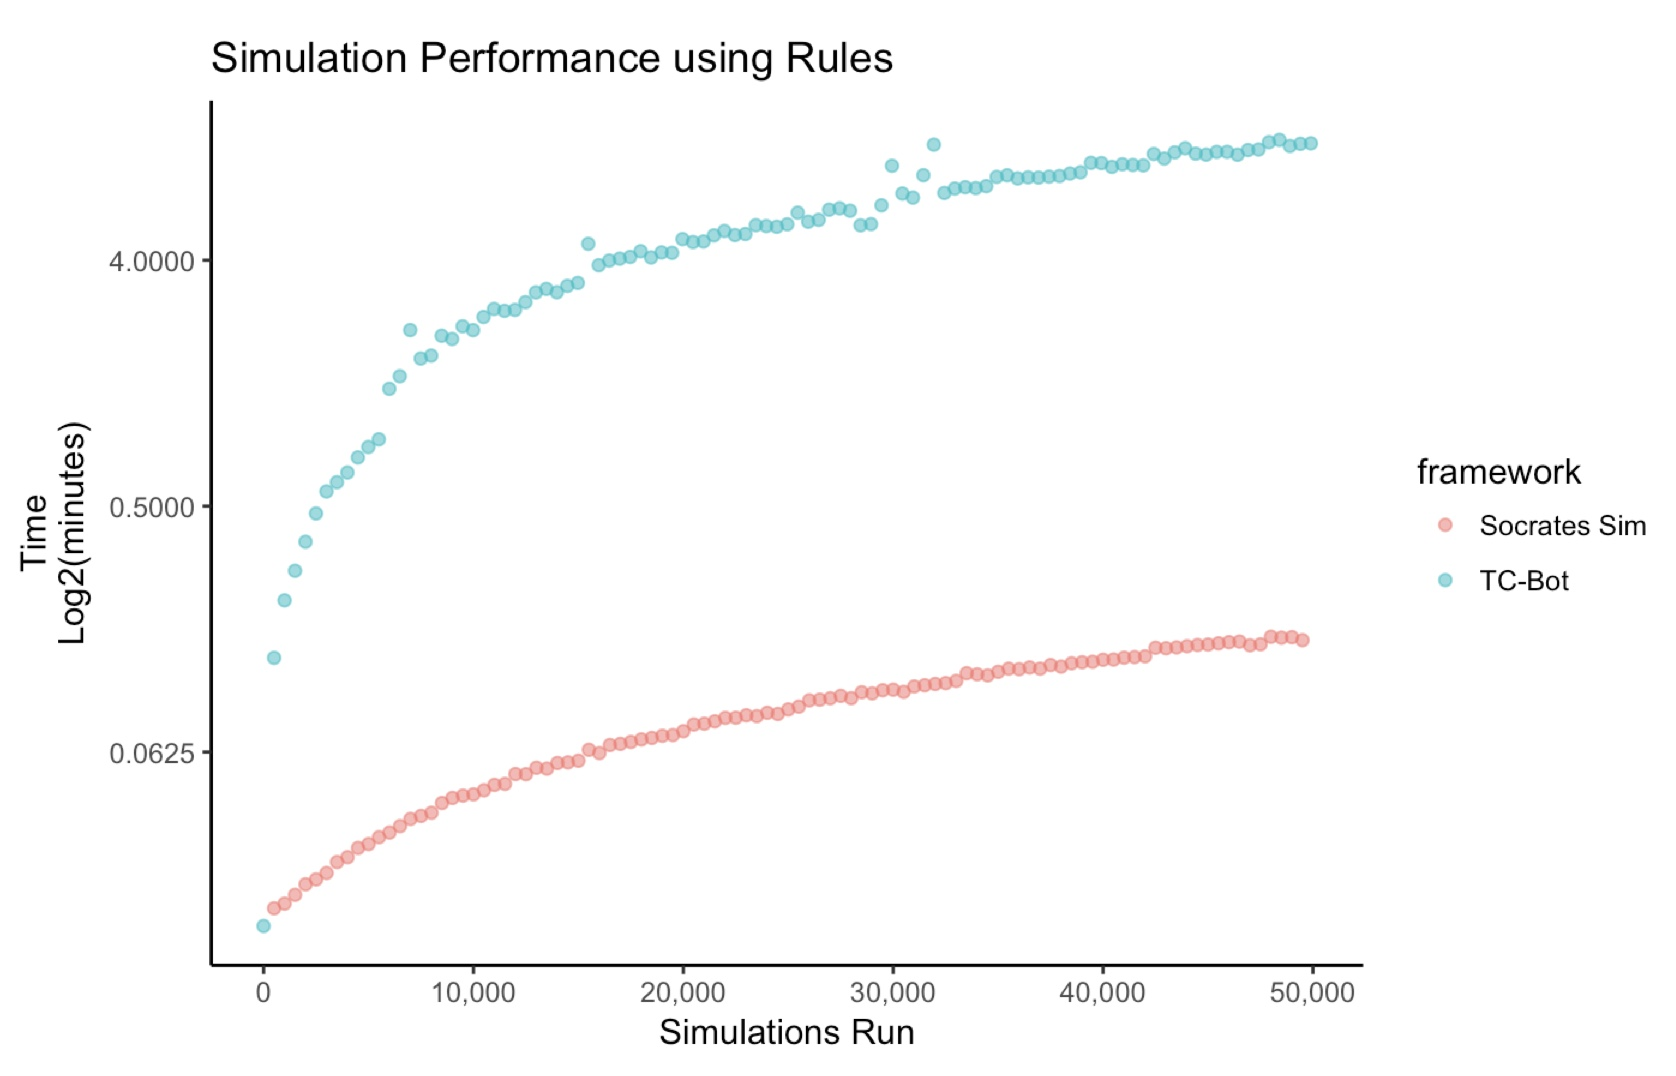
\includegraphics[width=\linewidth]{diagrams/rules_perf_test.jpeg}
	\caption{ Runtime of Socrates Sim vs TC-Bot with rule based user simulator.}
\end{figure}

For the first two tests, we compare the performance of end-to-end dialog simulations using a rules-based approach. For both frameworks, we use the movie booking use case. In the Socrates Simulator, both the dialog agent and user simulator are rules-based speakers and have rules-based nlu and nlg modules. In TC-Bot, the user simulator is rules-based and the dialog agent is a DQNN neural model that is being trained on a reward signal after each simulation round.  Both frameworks have a \textit{O(N)} runtime as the simulation sizes grew, as shown in Figure \ref{fig:rules_test}. However, Socrates Sim performed overall more efficiently, taking on average about 1 minute and 51 seconds to run 50,000 simulations. In contrast, TC-Bot took on average 10 minutes and 44 seconds. A large part of this can be attributed to the fact that TC-Bot tightly couples training the dialog agent with the dialog simulation. That is, after each round, TC-Bot runs stochastic gradient descent on the reward function in order to inform the dialog agent's action in the proceeding round. 

For the next two tests, we compare the performances of both frameworks using model-based actors. As with the first two experiments, we are evaluating in the movie booking use case. For Socrates Sim, we initially use the OpenNMT trained nlu and nlg module for the user simulator and dialog agent. Since OpenNMT does not support programmatic access, our initial performance tests were very poor. It took Socrates Sim about 50 minutes to run 1,000 simulations. Each call to OpenNMT required launching a new subprocess, invoking OpenNMT anew, and running the prediction. 

A preloaded model in memory would be more efficient. Therefore we switched to evaluating the performance of Socrates Sim using the \cite{brownlee_2017} neural machine translations models. The benefit of this model is that it can be invoked programmatically. At the very initial load, neural models (serialized as hd5 files) are loaded into memory. Each call to the model involved a small preprocessing cost and an additional cost to do a forward pass through the network.  On average, it took about 1 minute and 21 seconds to run 1,000 simulations. In contrast, we find that TC-Bot does perform much more efficiently. While its growth is still linear, it can run 1,000 simulations in about 30 seconds. For running neural models, TC-Bot is about 3 times faster. 

\begin{figure}[h!]
	\centering
	\label{fig:nm_test}
	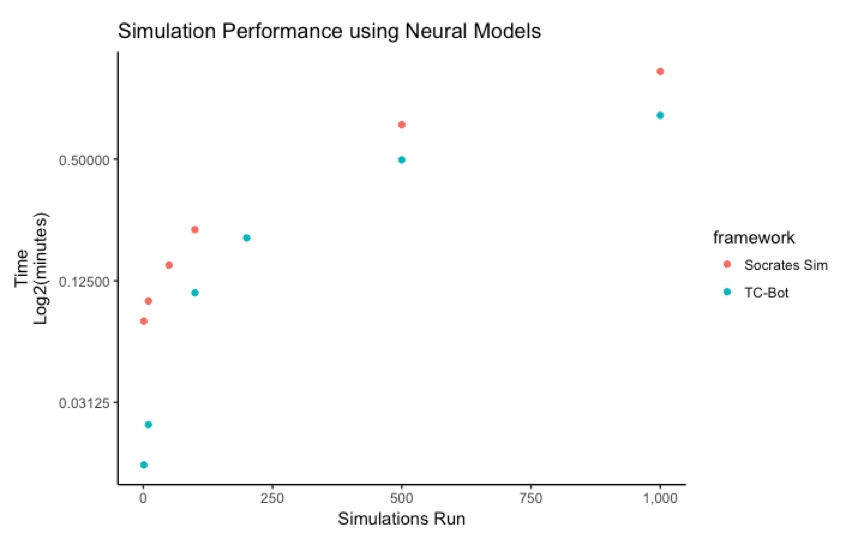
\includegraphics[width=\linewidth]{diagrams/neural_perf_test.jpeg}
	\caption{ Runtime of Socrates Sim vs TC-Bot with model-based user simulator.}
\end{figure}

 Finally, our last set of experiments involve testing runtime performance across domains. As TC-Bot is hard-coded for the movie booking use case, it was not included in our performance tests. In Figure \ref{fig:perf_cd_test}, we see that there is variation between domains. Both have linear growth, though the movie domain performs more efficiently, taking about 30 seconds to generate 50,000 simulations. What we find is that the overall performance of the framework is tied to the complexity of the domain and speaker classes. From a general usability point of view, we assert that framework scales predictably and is usable. End-to-end, it takes about two minutes to run 50,000 simulations for the restaurant domain, which is reasonable. 
 
  \begin{figure}[h!]
 	\label{fig:perf_cd_test}
 	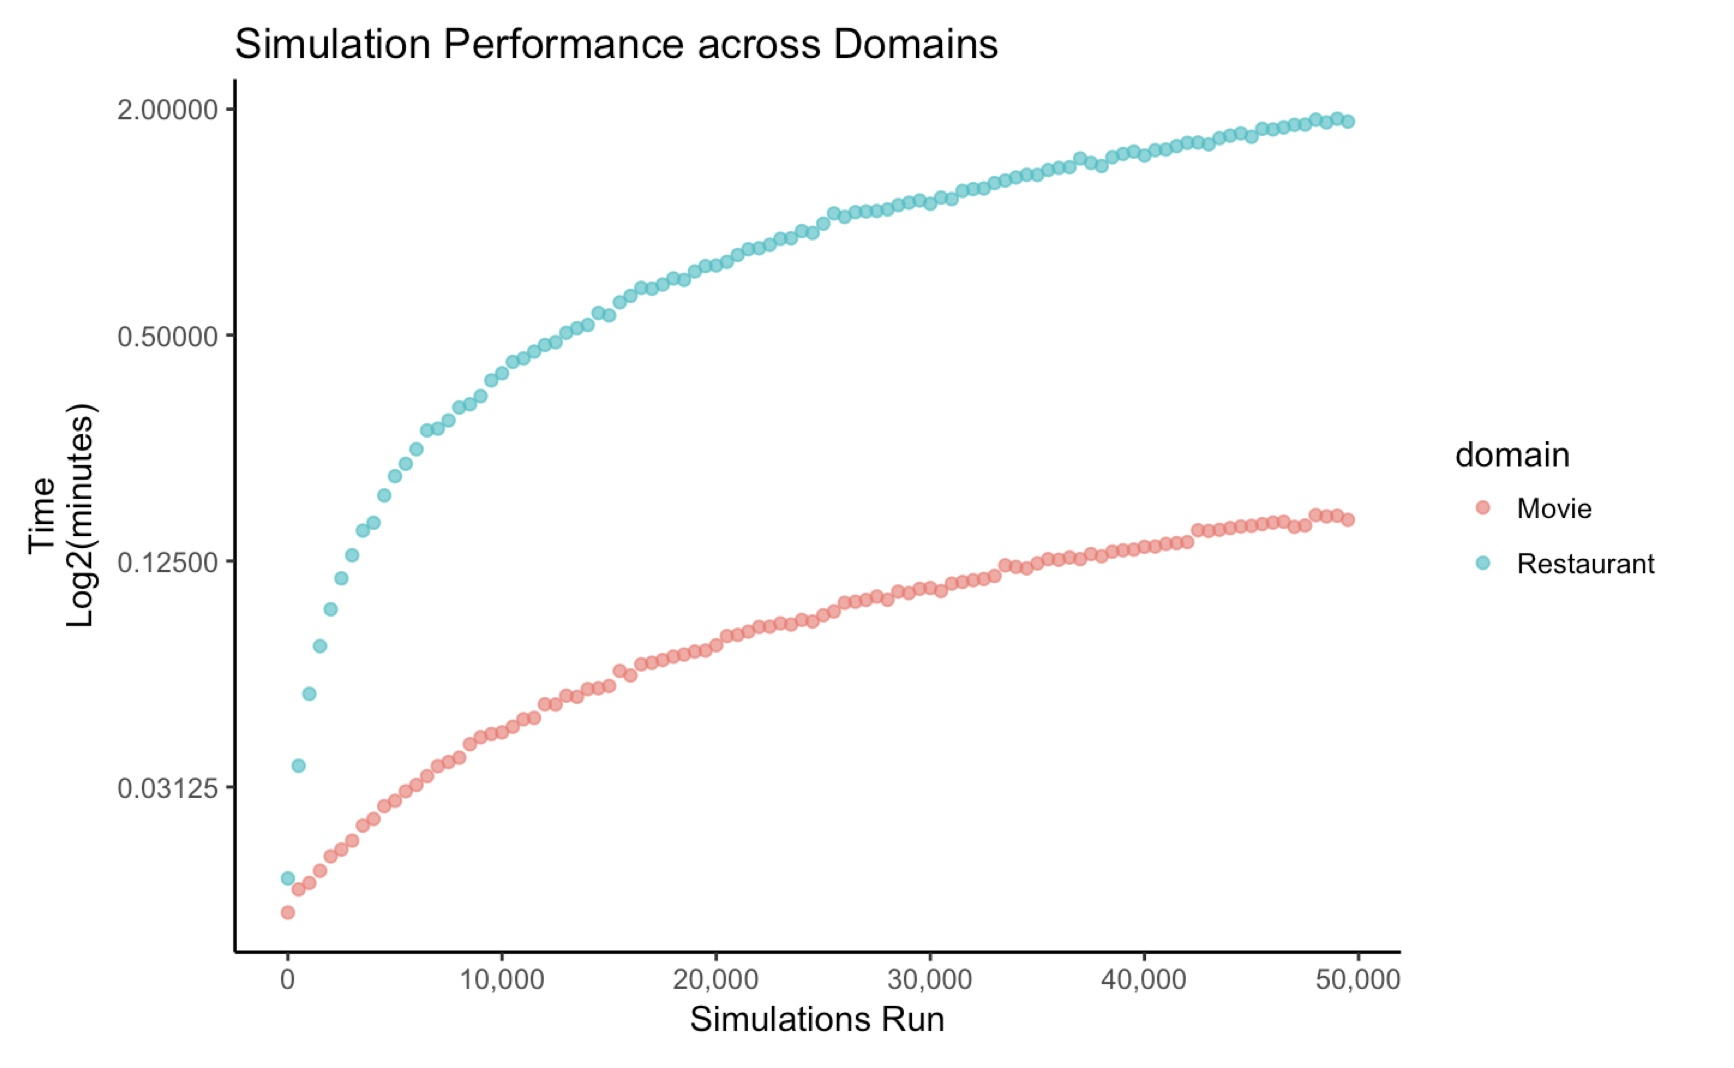
\includegraphics[width=\linewidth]{diagrams/domain_perf.jpeg}
 	\caption{ Runtime performance across domains.}
 \end{figure}

Growth is linear across all frameworks and domains. In the table below, we measure the average cost per simulation and rank all the framework/domain combinations from fastest to the slowest. The rules-based models for Socrates Sim significantly outperforms TC-Bot. In contrast, the model-based TC-Bot is about three times faster that Socrates Sim. Finally, rules-based approaches, in general, are more efficient to run. 

\begin{figure}[h!]
	\centering
	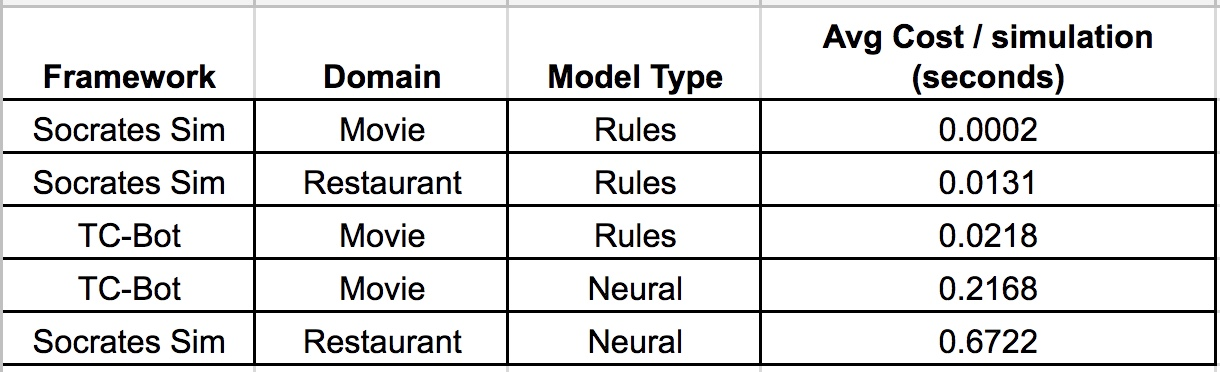
\includegraphics[width=\linewidth]{diagrams/avg_cost.jpeg}	
	\caption{ Average time to run a single simulation.}
	\label{fig:avg_cost}
\end{figure}

 There is an opportunity to further improve overall performance. As the simulations can run independently, we can introduce multi-threading and leverage the multi-core cpus for parallel processing. The dialog manager can be extended to support a thread pool and spawn multiple threads to run simulations in parallel. This could significantly improve performance if the researcher needs to generate hundreds of thousands or millions of simulations.  

\section{Memory Consumption Experiment and Results}

The next set of tests involve measuring maximum memory consumption of the framework when generating multiple dialog simulations. The goal is to show that Socrates Simulator consumes memory reasonably and is usable. Like the performance tests above, we ran a total of 6 tests to evaluate memory consumption. Four tests were on the Socrates Sim framework and two on the TC-Bot framework.

To measure memory consumption, we used the Python based \textit{memory-profiler} tool. The tool is invoked via command lined and runs the program to be evaluated as an internal sub-process. Over the duration of the observed program's runtime, \textit{memory-profiler} uses the \textit{psustil} tool to probe the operating system for information about CPU usage, running processes, and resource utilization. \textit{Memory-profiler} will log memory usage at predefined increments until the program finishes running. 

\begin{figure}[h!]
	\label{fig:mem_usage_rules}
	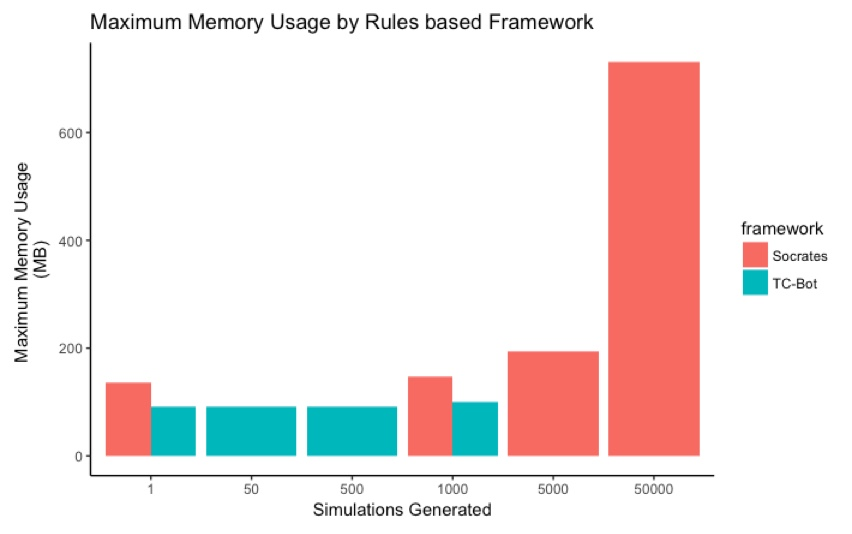
\includegraphics[width=\linewidth]{diagrams/mem_usage_rules.jpeg}
	\caption{ Memory usage of Socrates Sim vs TC-Bot with rule based user simulator.}
\end{figure}

For the first test, we looked at the maximum memory usage of both frameworks when using rule-based actors for the movie domain. Figure \ref{fig:mem_usage_rules} shows relative performance of both frameworks. TC-Bot performs significantly better, capping at about 150 MB of overall memory usage over the course all simulations run. Running up to 5,000 simulations, Socrates Sim uses under 200 MB of memory. At the 50,000 simulations, memory usage does significantly increase to about 700 MB. It is worth noting that this much memory is only utilized at the tail end of Socrates Sim's runtime. This likely due to the fact that the dialog manager has not serialized the generated dialogs and is holding them in memory until all simulations have run.  

\begin{figure}[h!]
		\centering
	\label{fig:mem_usage_nm}
	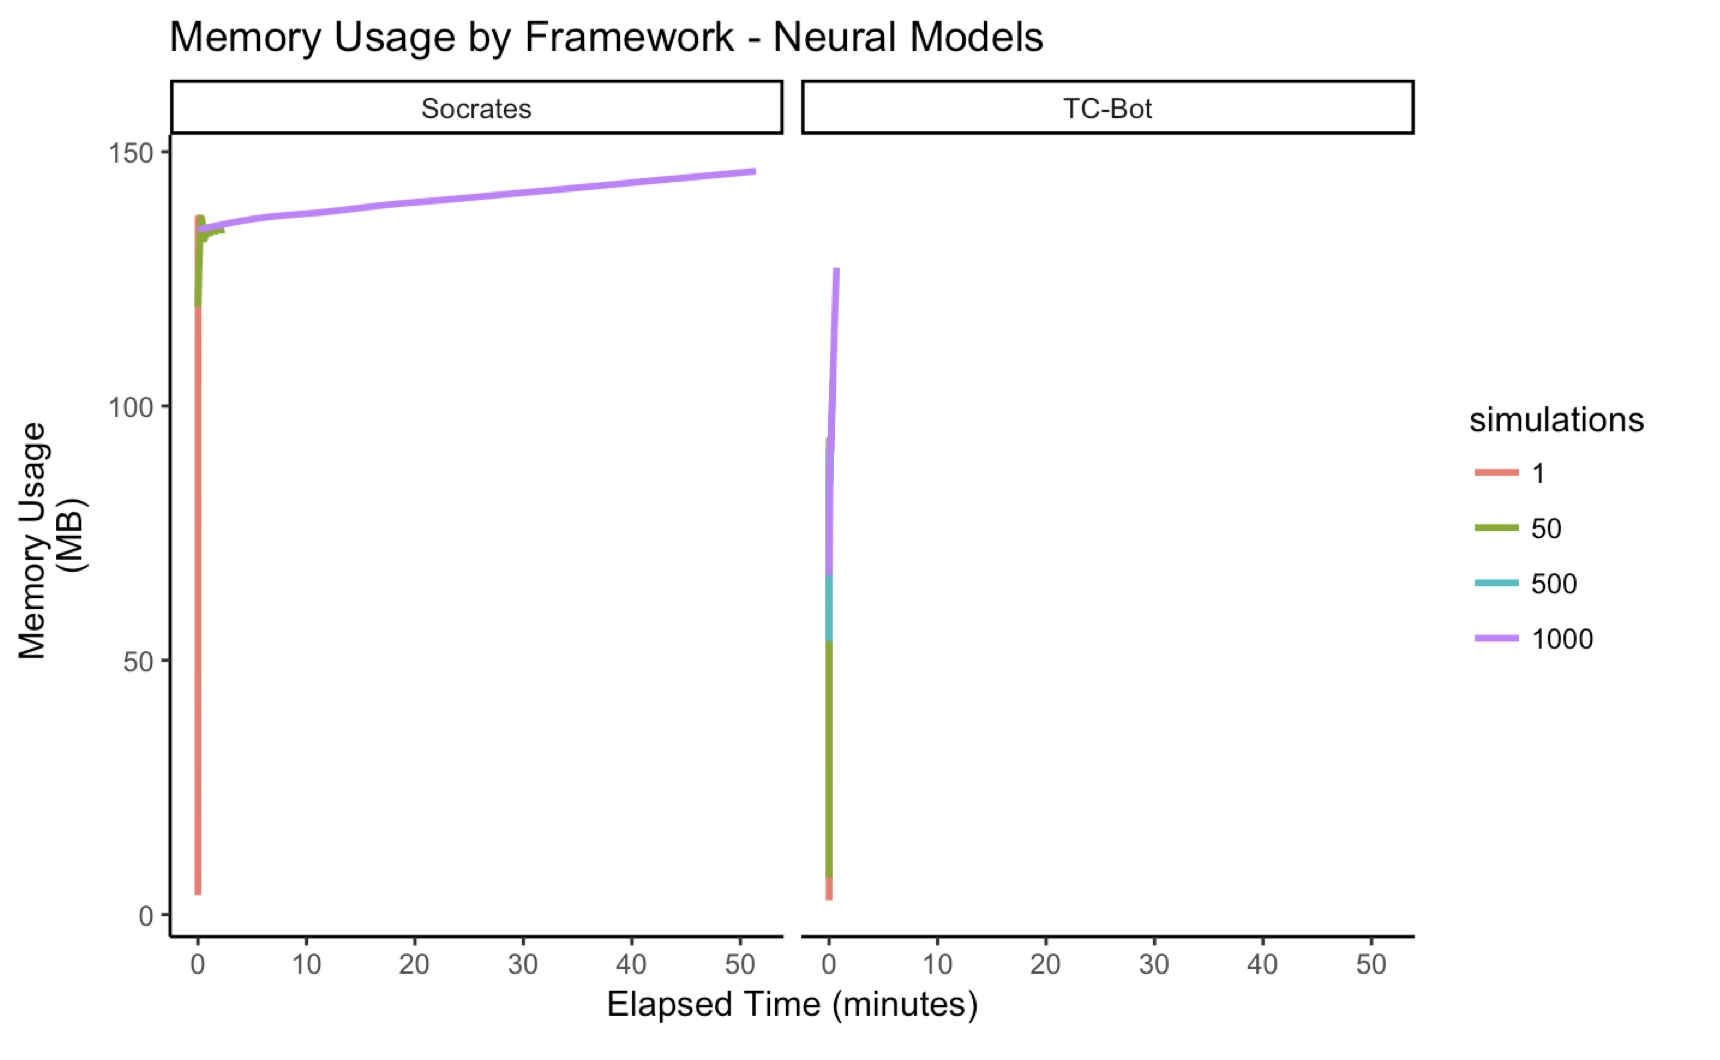
\includegraphics[width=\linewidth]{diagrams/mem_usage_neural.jpeg}
	\caption{ Memory usage of Socrates Sim vs TC-Bot with model-based user simulator. }
\end{figure}

In Figure \ref{fig:mem_usage_nm}, we see the results for memory consumption when using neural models. Note, that we used the restaurant domain for reasons explained above. Overall, both TC-Bot and Socrates Sim use a little under 150 MB. While runtime performance is drastically different, with TC-Bot running more efficiently overall, both frameworks have similar memory usage patterns. 

Finally, in Figure \ref{fig:mem_usage_cd}, we see the results for memory usage across the restaurant and movie domains for Socrates Sim. Under 10,000 simulations, we found total memory usage caps around 250 MB. 

\begin{figure}[h!]
		\centering
	\label{fig:mem_usage_cd}
	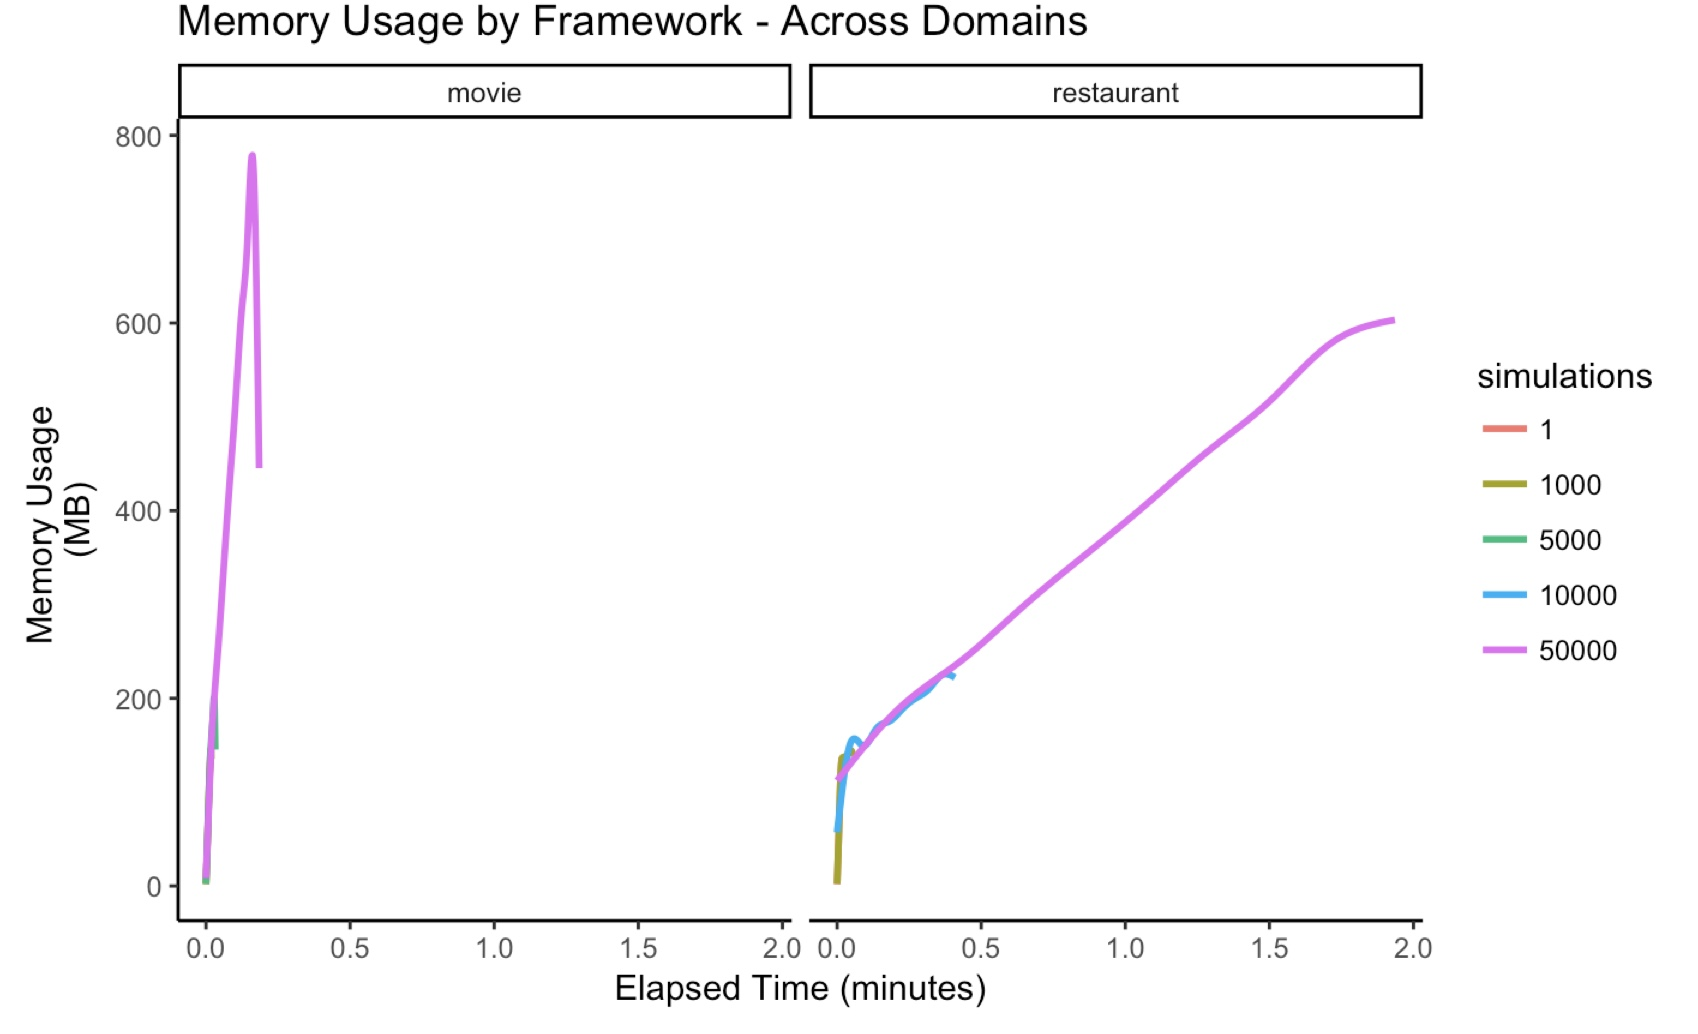
\includegraphics[width=\linewidth]{diagrams/mem_usage_domains.jpeg}
	\caption{ Memory usage across domains for Socrates Sim.}
\end{figure}

All the tests reveal a small oversight in the Socrates Simulator design. The tests show that memory usage grows linearly with the number of simulations run. This is due to the fact the dialog manager does not serialize the generated dialogs until all simulations are run. This is a minor design choice, which can be updated to have the dialog manager periodically serialize the queue of generated dialogs and reset the queue. 

Accounting for the serialization issue, the overall memory usage for Socrates Sim is reasonable. In small simulations (under 50,000), Socrates Sim has a similar memory usage profile to TC-Bot. We believe Socrates Simulator is usable and provides predictable performance and memory utilization. For rules-based use case, Socrates Sim is quite efficient. Accounting for the complexity of the rules, the researcher is able to run thousands of simulations in a matter of minutes. Overall, both the performance tests and memory utilization tests show that Socrates Simulator can be used for most reasonable use cases. 
%%% Local Variables: 
%%% mode: latex
%%% TeX-master: "main"
%%% End: 




\chapter{Sequence Analysis Tools and Applications}
\label{chap:sequence}

%http://en.wikipedia.org/wiki/Pandemic_H1N1/09_virus

...


\section{Needleman-Wunsch Implementation}
\label{sec:nw}

...


\subsection{Global Sequence Alignment}
\label{sec:seqglobal}

...

\subsection{Longest Common Subsequence (LCS)}
\label{sec:lcs}


...

Essentially the first step of \algor{LCS} performs this
recursion:
\begin{eqnarray}
S_{0,j} &=& 0\\
S_{i,0} &=& 0\\
S_{i,j} &=& \max
\begin{cases}
  S_{i,j-1} & \\
  S_{i-1,j} & \\
  S_{i-1,j-1} + 1 & \textrm{if } A_i = B_j
\end{cases}
\end{eqnarray}
\addmyequations{Longest Common Subsequence Recursion}

...

The pseudocode of \algor{LCS} is shown in Algorithm~\ref{algo:LCS}.

...


\begin{algorithm}
  \caption{\algor{LCS}($A_{0..n},B_{0..m}$)}
  \label{algo:LCS}
\begin{lstlisting}[language=Algorithm]
$S_{i,j} \as 0 $ for all $i = 0$ or $j = 0$		{set first row and first column to $0$}
$T_{i,j} \as \sym{UP}$ for all $i,j$			{pointing up by default}

for $i \as 1$ to $n$ do
   for $j \as 1$ to $m$ do
      $S_{i,j} = \max 
\begin{cases}
  S_{i,j-1} & \\
  S_{i-1,j} & \\
  S_{i-1,j-1} + 1 & \textrm{if } A_i = B_j
\end{cases}$
      $T_{i,j} = 
\begin{cases}
  \sym{LEFT} & \textrm{if } S_{i,j} = S_{i,j-1}\\
  \sym{UP} & \textrm{if } S_{i,j} = S_{i-1,j}\\
  \sym{DIAGONAL} & \textrm{if } S_{i,j} = S_{i-1,j-1} + 1
\end{cases}$
$\algor{Backtrace}(A,T, n, m)$

function $\algor{Backtrace}(A_{0..n},T_{0..n\times 0..m}, i, j)$
   if $i = 0$ or $j = 0$ then
      return
   if $T_{i,j} = \sym{DIAGONAL}$ then
      $\algor{Backtrace}(A,T_{n,m}, i-1, j-1)$
      print $A_i$
   else if $T_{i,j} = \sym{UP}$ then
      $\algor{Backtrace}(A,T, i-1, j)$
   else 
      $\algor{Backtrace}(A,T, i, j-1)$
end
\end{lstlisting}
\end{algorithm}




%%% Local Variables: 
%%% mode: latex
%%% TeX-master: "main"
%%% End: 



\chapter{Conclusion}
\label{chap:conclusions}

\section{ Known Limitations and Suggestions for Future Work}
\label{sec:issues} 

Overall, the framework works as intended. One key limitation was discovered during performance testing. We found that our serialization strategy causes the framework to consume memory linearly as the number of simulations increase. This occurs because the dialog manager waits until all simulations are run before dumping the generated dialog history. As a result, the in-memory json representation grows linearly with each incremental simulation run. The remedy for this is straightforward. The dialog manager can store the dialog history in a fixed size buffer that serializes to storage when it is full. 

We also saw limitations around neural mode runtime performance and general qualitative performances in the context of nlg and nlu. The focus of this project was the engineering and development of the simulation framework. Unfortunately, we did not have time to explore how to optimize neural architectures to support our use cases. This is an exciting and active area of research and offers many interesting avenues for further inquiry.

In a related vein, we were unable to support reinforcement learning and incorporate online training of the dialog agent in our framework. There is fascinating value to extend the framework to provide reward signals and support live training of the dialog agent based off of the feedback from the user simulator. 

Finally, there is an opportunity to extend Socrates Sim by adding in a visual interface. Currently, it is command line driven. The framework is developed with modularity in mind. We have abstracted the domain logic from the implementation layer. As a result, a visual front end can be developed for Socrates Sim without modifying the underlying framework.

\section{Lessons Learned}
\label{sec:lessons}

This thesis was our first foray into task completion dialog research and statistical language understanding. While we ultimately approached this domain from an engineering perspective, we did gain a better understanding of the active research challenges and model-based approaches. Our understanding of the capabilities and limitations of neural network-based approaches was likewise enriched. 

From a software engineering perspective, the greatest challenge we ran into was walking the fine line between defining rigid conventions to ensure predictable usage versus allowing for more flexibility to empower the user. Often Socrates Sim was written and rewritten to accommodate marginal edge cases because our design choices tilted too far on the flexible side. Other times, in an effort reduce  manual coding for the end user, we tilted too far in the opposite direction and defined very rigid conventions. Our end takeaway was that it often helps to take a step back and list out the various use cases. If you can make assumptions that captures 60\% to 80\% of those use cases, then developing defined conventions is very valuable. In fact, it reduces the friction and learning curve to understand and use your tools.

Additionally, this project was a great deep dive into using the Python language for a larger scale project. One of the persistent challenges with Python is due to dynamic typing. In large projects, it is hard track bugs as objects and variable are mutable and not strictly typed. The ability to explore Python 3.5's type hinting capabilities was useful and illuminating, especially since type hinting provides a way to raise the quality of your Python code base to meet software engineering best practices and norms.

\section{Summary}

In summary, we have demonstrated the design and implementation of an end-to-end dialog simulation framework that supports task-completion dialog research. In chapter 2, we detailed a modular architecture that can be re-targeted to new domains and scaled efficiently. Central to this design were four key components. The first was the speaker abstract base class, which provides a unified interface for external user simulators and dialog agents to communicate with the framework in a standardized manner. The second was the codification of the dialog domain, where dialog acts, inform and request slots and slot values, and other pertinent information to the domain is captured. The dialog domain object is made available to the dialog manager, dialog agent, and user simulator. The third important component was the standardization of ancillary communication components like the dialog action object. Specifically, we extend and formally implement as classes the user goal and user agenda described in \cite{Schatzmann2009TheHA} to support the development of a user simulator. The final component is the dialog manager, which tracks, evaluates, and serializes simulated dialogs. 

In chapter 3, we described the general process of implementing Socrates Sim. We highlighted our configuration-first philosophy, inspired by \cite{Gardner_allennlp}, which allowed for the framework to more easily generalize to new domains. Specifically, we called out the use of the simulation configuration file. The configuration file allows the researcher to integrate an external user simulator, dialog agent, and domain into the framework. We also demonstrated modularity by supporting the dynamic loading of the nlg and nlu modules.

In chapter 4 and 5 we explored in detail how Socrates Sim was adapted for the restaurant recommendation and movie booking domains. We detailed the development of dialog domain, dialog agent, and user simulators for both domains. We showed specifically how Socrates Sim was able to support new domains and nlg/nlu models with the use of configuration files and require no code update to the underlying framework and dialog manager. In doing so, we were able to demonstrate that the framework is retargetable. 
  
In chapter 6, we described how Socrates Sim was developed. We highlighted the tools, programming language, and other development specific choices made while developing Socrates Sim. In chapter 7, we provided evidence that Socrates Sim is usable and scale efficiently. Multiple performance tests were run to evaluate the runtime efficiency and memory consumption of Socrates Sim as it ran an increasing number of simulations. We used TC-Bot (\cite{li_end_to_end}) as a benchmark to evaluate performance. 

The testing confirmed that Socrates Sim scales efficiently and predictably running up to 50,000 simulations. While Socrates Sim does scale linearly as the required number of simulations increase, performance does not degrade until you exceed 100,000 simulations. The average cost of running rules-based user simulators in Socrates Sim is between .0002 to .0131 seconds. You are able to simulate 50,000 dialogs in under two minutes, which far exceeds the performance of TC-Bot. We also find there is an opportunity for improvement in improving model-based simulations in Socrates Sim. Objectively, the average cost for a model-based simulation is .6722 seconds and it takes about one hour to run 50,000 simulations. In contrast, the average cost per simulation for TC-Bot's .2168 seconds. TC-Bot is able to run 50,00 simulations in about 30 seconds. 
 
In conclusion, we have developed a framework that supports multi-domain task completion research. We have demonstrated the framework's ability to support new domains without changing the underlying code. Additionally, our performance tests reveal that Socrates Sim scales efficiently and is generally usable. Our hope is this project can provide the foundations to support end-to-end task completion research and can be extended to provide new value by the community.

%%% Local Variables: 
%%% mode: latex
%%% TeX-master: "main"
%%% End: 



\clearpage
\phantomsection
\addcontentsline{toc}{chapter}{References}
\renewcommand{\bibname}{References}
\bibliographystyle{apalike2}
\bibliography{main}


% ------------------------------------------------------------
% APPENDIX

\newpage
\appendix



\clearpage
\phantomsection
\printglossary

\clearpage

% CODE APPENDICES
% should be single space
% each code package, and each code file, should begin on a new page
\singlespacing
\phantomsection

\chapter{Application Code}
%\minitoc
\label{chap:code}
%%\addcontentsline{toc}{chapter}{Appendix B\hspace*{1.6em}Probability and Statistics}

%\section{Java Code}
%\label{sec:javacode}
%\subsection{package account}

\lstinputlisting[language=Java,caption={/account/business/AccountManager.java},label={/account/business/AccountManager.java}]{./src/main/java/com/myapp/magi/account/business/AccountManager.java}
\afterpage{\clearpage\lstinputlisting[language=Java,caption={/account/business/AccountManagerBean.java},label={/account/business/AccountManagerBean.java}]{./src/main/java/com/myapp/magi/account/business/AccountManagerBean.java} }
\clearpage\newpage

\subsection{package utils}

...

\clearpage\newpage


%\clearpage
%\newpage
%\section{JSF Code}
%\label{sec:jsfcode}
%\input{code_jsf}

%\clearpage
%\newpage
%\section{XML Code}
%\label{sec:xmlcode}
%\input{code_xml}


%\clearpage
%\newpage
%\section{R Code}
%\label{sec:rcode}
%\input{code_r}

%\clearpage
%\newpage
%\section{Python Code}
%\label{sec:pythoncode}
%\input{code_python}




%%% Local Variables: 
%%% mode: latex
%%% TeX-master: "main"
%%% End: 



\end{document}


%%% Local Variables: 
%%% mode: latex
%%% TeX-master: t
%%% End: 
